% Options for packages loaded elsewhere
\PassOptionsToPackage{unicode}{hyperref}
\PassOptionsToPackage{hyphens}{url}
%
\documentclass[
]{article}
\usepackage{lmodern}
\usepackage{amssymb,amsmath}
\usepackage{ifxetex,ifluatex}
\ifnum 0\ifxetex 1\fi\ifluatex 1\fi=0 % if pdftex
  \usepackage[T1]{fontenc}
  \usepackage[utf8]{inputenc}
  \usepackage{textcomp} % provide euro and other symbols
\else % if luatex or xetex
  \usepackage{unicode-math}
  \defaultfontfeatures{Scale=MatchLowercase}
  \defaultfontfeatures[\rmfamily]{Ligatures=TeX,Scale=1}
\fi
% Use upquote if available, for straight quotes in verbatim environments
\IfFileExists{upquote.sty}{\usepackage{upquote}}{}
\IfFileExists{microtype.sty}{% use microtype if available
  \usepackage[]{microtype}
  \UseMicrotypeSet[protrusion]{basicmath} % disable protrusion for tt fonts
}{}
\makeatletter
\@ifundefined{KOMAClassName}{% if non-KOMA class
  \IfFileExists{parskip.sty}{%
    \usepackage{parskip}
  }{% else
    \setlength{\parindent}{0pt}
    \setlength{\parskip}{6pt plus 2pt minus 1pt}}
}{% if KOMA class
  \KOMAoptions{parskip=half}}
\makeatother
\usepackage{xcolor}
\IfFileExists{xurl.sty}{\usepackage{xurl}}{} % add URL line breaks if available
\IfFileExists{bookmark.sty}{\usepackage{bookmark}}{\usepackage{hyperref}}
\hypersetup{
  hidelinks,
  pdfcreator={LaTeX via pandoc}}
\urlstyle{same} % disable monospaced font for URLs
\usepackage{longtable,booktabs}
% Correct order of tables after \paragraph or \subparagraph
\usepackage{etoolbox}
\makeatletter
\patchcmd\longtable{\par}{\if@noskipsec\mbox{}\fi\par}{}{}
\makeatother
% Allow footnotes in longtable head/foot
\IfFileExists{footnotehyper.sty}{\usepackage{footnotehyper}}{\usepackage{footnote}}
\makesavenoteenv{longtable}
\usepackage{graphicx}
\makeatletter
\def\maxwidth{\ifdim\Gin@nat@width>\linewidth\linewidth\else\Gin@nat@width\fi}
\def\maxheight{\ifdim\Gin@nat@height>\textheight\textheight\else\Gin@nat@height\fi}
\makeatother
% Scale images if necessary, so that they will not overflow the page
% margins by default, and it is still possible to overwrite the defaults
% using explicit options in \includegraphics[width, height, ...]{}
\setkeys{Gin}{width=\maxwidth,height=\maxheight,keepaspectratio}
% Set default figure placement to htbp
\makeatletter
\def\fps@figure{htbp}
\makeatother
\setlength{\emergencystretch}{3em} % prevent overfull lines
\providecommand{\tightlist}{%
  \setlength{\itemsep}{0pt}\setlength{\parskip}{0pt}}
\setcounter{secnumdepth}{-\maxdimen} % remove section numbering

\author{}
\date{}

\begin{document}

{OpenBikeSensor Bauanleitung}

{}

{Bauteile:}

{HC-SR04P Sensor }

{Hinweis: Die Sensoren messen per Ultraschall den Abstand zum
überholenden Fahrzeug und auch den Abstand zu parkenden Fahrzeugen. Ihr
benötigt zwei Stück pro OBS.}

{\href{https://www.google.com/url?q=https://www.aliexpress.com/item/33039149738.html\&sa=D\&ust=1588976963766000}{https://www.aliexpress.com/item/33039149738.html}}

{}

{5-pin XS9 Aviation Connector }

{Hinweis: Die Push-Pull Rundsteckverbindung ist die Verbindung zwischen
dem OBS und dem Kabel zum Push Button am Lenker. }

{\href{https://www.google.com/url?q=https://www.aliexpress.com/item/32512693653.html\&sa=D\&ust=1588976963767000}{https://www.aliexpress.com/item/32512693653.html}}

{}

{12mm Push Button}

{Hinweis: Dieser Button ist die Drucktaste am Lenker mit dem jeder echte
Überholvorgang eines Fahrzeugs bestätigt werden soll.}

{\href{https://www.google.com/url?q=https://www.aliexpress.com/item/4000295670163.html\&sa=D\&ust=1588976963768000}{https://www.aliexpress.com/item/4000295670163.html}}

{}

{0.96 inch OLED Display}

{Hinweis: Das Display am Lenker zeigt euch den Überholabstand in
Zentimeter an. Das Display in dieser Form ist nicht wasserfest. Bei
Regen bitte Folie über das Display kleben!}

{\href{https://www.google.com/url?q=https://www.aliexpress.com/item/32896971385.html\&sa=D\&ust=1588976963769000}{https://www.aliexpress.com/item/32896971385.html}}

{}

{18650-LiFePo Battery}

{Hinweis: Der Akku für den OBS. Nach letzten Messungen hält der Akku gut
einen Tag. }

{\href{https://www.google.com/url?q=https://www.akkuteile.de/lifepo-akkus/18650/a123-apr18650m-a1-1100mah-3-2v-3-3v-lifepo4-akku/a-1006861/\&sa=D\&ust=1588976963770000}{https://www.akkuteile.de/lifepo-akkus/18650/a123-apr18650m-a1-1100mah-3-2v-3-3v-lifepo4-akku/a-1006861/}}

{}

{TP5000 LiFePo-Charger}

{Hinweis: Lademodul mit Micro USB Anschluss. }

{\href{https://www.google.com/url?q=https://www.ebay.de/itm/122164745507\&sa=D\&ust=1588976963771000}{https://www.ebay.de/itm/122164745507}}

{\href{https://www.google.com/url?q=https://www.aliexpress.com/item/4000310107151.html\&sa=D\&ust=1588976963771000}{https://www.aliexpress.com/item/4000310107151.html}}

{}

{USB-C Lademodul}

{\href{https://www.google.com/url?q=https://www.ebay.de/itm/173893903484\&sa=D\&ust=1588976963772000}{https://www.ebay.de/itm/173893903484}}

{}

{LiFePo Protection Board}

{\href{https://www.google.com/url?q=https://www.ebay.de/i/202033076322?ul_noapp\%3Dtrue\&sa=D\&ust=1588976963773000}{https://www.ebay.de/i/202033076322?ul\_noapp=true}}

{}

{GPS-Modul}

{GYGPS6MV2 GPS Module Mini Antenna}

{\href{https://www.google.com/url?q=https://www.ebay.de/itm/GPS-NEO-6M-7M-8M-GY-GPS6MV2-Module-Aircraft-Flight-Controller-For-Arduino/272373338855\&sa=D\&ust=1588976963774000}{https://www.ebay.de/itm/GPS-NEO-6M-7M-8M-GY-GPS6MV2-Module-Aircraft-Flight-Controller-For-Arduino/272373338855}}

{}

{}

{ESP32}

{\href{https://www.google.com/url?q=https://www.az-delivery.de/collections/bestseller/products/esp32-developmentboard\&sa=D\&ust=1588976963775000}{https://www.az-delivery.de/collections/bestseller/products/esp32-developmentboard}}

{}

{}

{}

{}

{Inhaltsverzeichnis}

{Materialliste}

{Kabel: jetzige Version, alles 0,25mm}{2}{~}

{}

\protect\hypertarget{t.9a815b74fcc604715e7feb03f2d81a08b49f1f51}{}{}\protect\hypertarget{t.0}{}{}

\begin{longtable}[]{@{}llll@{}}
\toprule
\endhead
\begin{minipage}[t]{0.22\columnwidth}\raggedright
{Bauteil}\strut
\end{minipage} & \begin{minipage}[t]{0.22\columnwidth}\raggedright
{ESP32}\strut
\end{minipage} & \begin{minipage}[t]{0.22\columnwidth}\raggedright
{Masse und VCC}\strut
\end{minipage} & \begin{minipage}[t]{0.22\columnwidth}\raggedright
{Sonstige}\strut
\end{minipage}\tabularnewline
\begin{minipage}[t]{0.22\columnwidth}\raggedright
{Ultraschallsensoren}\strut
\end{minipage} & \begin{minipage}[t]{0.22\columnwidth}\raggedright
{4 x 12cm}\strut
\end{minipage} & \begin{minipage}[t]{0.22\columnwidth}\raggedright
{2 x 12cm}\strut
\end{minipage} & \begin{minipage}[t]{0.22\columnwidth}\raggedright
{direkte Verbindung zwischen Sensoren}

{2x 3,5cm}\strut
\end{minipage}\tabularnewline
\begin{minipage}[t]{0.22\columnwidth}\raggedright
{SD}\strut
\end{minipage} & \begin{minipage}[t]{0.22\columnwidth}\raggedright
{4 x 10cm}\strut
\end{minipage} & \begin{minipage}[t]{0.22\columnwidth}\raggedright
{2 x 10cm}\strut
\end{minipage} & \begin{minipage}[t]{0.22\columnwidth}\raggedright
{direkte Verbindung Masse 1x 2,5cm}\strut
\end{minipage}\tabularnewline
\begin{minipage}[t]{0.22\columnwidth}\raggedright
{GPS}\strut
\end{minipage} & \begin{minipage}[t]{0.22\columnwidth}\raggedright
{2x 9,5cm}\strut
\end{minipage} & \begin{minipage}[t]{0.22\columnwidth}\raggedright
{2x 9,5cm}\strut
\end{minipage} & \begin{minipage}[t]{0.22\columnwidth}\raggedright
{}\strut
\end{minipage}\tabularnewline
\begin{minipage}[t]{0.22\columnwidth}\raggedright
{}\strut
\end{minipage} & \begin{minipage}[t]{0.22\columnwidth}\raggedright
{}\strut
\end{minipage} & \begin{minipage}[t]{0.22\columnwidth}\raggedright
{}\strut
\end{minipage} & \begin{minipage}[t]{0.22\columnwidth}\raggedright
{}\strut
\end{minipage}\tabularnewline
\begin{minipage}[t]{0.22\columnwidth}\raggedright
{ESP-VCC und GND}\strut
\end{minipage} & \begin{minipage}[t]{0.22\columnwidth}\raggedright
{}\strut
\end{minipage} & \begin{minipage}[t]{0.22\columnwidth}\raggedright
{}\strut
\end{minipage} & \begin{minipage}[t]{0.22\columnwidth}\raggedright
{2x8cm}\strut
\end{minipage}\tabularnewline
\begin{minipage}[t]{0.22\columnwidth}\raggedright
{Buchse}\strut
\end{minipage} & \begin{minipage}[t]{0.22\columnwidth}\raggedright
{3 x 13cm}\strut
\end{minipage} & \begin{minipage}[t]{0.22\columnwidth}\raggedright
{2x 13cm}\strut
\end{minipage} & \begin{minipage}[t]{0.22\columnwidth}\raggedright
{}\strut
\end{minipage}\tabularnewline
\begin{minipage}[t]{0.22\columnwidth}\raggedright
{}\strut
\end{minipage} & \begin{minipage}[t]{0.22\columnwidth}\raggedright
{}\strut
\end{minipage} & \begin{minipage}[t]{0.22\columnwidth}\raggedright
{}\strut
\end{minipage} & \begin{minipage}[t]{0.22\columnwidth}\raggedright
{}\strut
\end{minipage}\tabularnewline
\begin{minipage}[t]{0.22\columnwidth}\raggedright
{Schalter}\strut
\end{minipage} & \begin{minipage}[t]{0.22\columnwidth}\raggedright
{}\strut
\end{minipage} & \begin{minipage}[t]{0.22\columnwidth}\raggedright
{}\strut
\end{minipage} & \begin{minipage}[t]{0.22\columnwidth}\raggedright
{2x6cm}\strut
\end{minipage}\tabularnewline
\begin{minipage}[t]{0.22\columnwidth}\raggedright
{Batterie-Schutzmodul}\strut
\end{minipage} & \begin{minipage}[t]{0.22\columnwidth}\raggedright
{}\strut
\end{minipage} & \begin{minipage}[t]{0.22\columnwidth}\raggedright
{}\strut
\end{minipage} & \begin{minipage}[t]{0.22\columnwidth}\raggedright
{2x2,5cm}\strut
\end{minipage}\tabularnewline
\begin{minipage}[t]{0.22\columnwidth}\raggedright
{Schutzmodul-Schalter / Masse}\strut
\end{minipage} & \begin{minipage}[t]{0.22\columnwidth}\raggedright
{}\strut
\end{minipage} & \begin{minipage}[t]{0.22\columnwidth}\raggedright
{}\strut
\end{minipage} & \begin{minipage}[t]{0.22\columnwidth}\raggedright
{2x 9cm}\strut
\end{minipage}\tabularnewline
\begin{minipage}[t]{0.22\columnwidth}\raggedright
{}\strut
\end{minipage} & \begin{minipage}[t]{0.22\columnwidth}\raggedright
{}\strut
\end{minipage} & \begin{minipage}[t]{0.22\columnwidth}\raggedright
{}\strut
\end{minipage} & \begin{minipage}[t]{0.22\columnwidth}\raggedright
{}\strut
\end{minipage}\tabularnewline
\begin{minipage}[t]{0.22\columnwidth}\raggedright
{Lademodul USB-C zu LiFePo-Lader}\strut
\end{minipage} & \begin{minipage}[t]{0.22\columnwidth}\raggedright
{}\strut
\end{minipage} & \begin{minipage}[t]{0.22\columnwidth}\raggedright
{}\strut
\end{minipage} & \begin{minipage}[t]{0.22\columnwidth}\raggedright
{2x3cm}\strut
\end{minipage}\tabularnewline
\begin{minipage}[t]{0.22\columnwidth}\raggedright
{}\strut
\end{minipage} & \begin{minipage}[t]{0.22\columnwidth}\raggedright
{}\strut
\end{minipage} & \begin{minipage}[t]{0.22\columnwidth}\raggedright
{}\strut
\end{minipage} & \begin{minipage}[t]{0.22\columnwidth}\raggedright
{}\strut
\end{minipage}\tabularnewline
\begin{minipage}[t]{0.22\columnwidth}\raggedright
{Stecker-Display}\strut
\end{minipage} & \begin{minipage}[t]{0.22\columnwidth}\raggedright
{}\strut
\end{minipage} & \begin{minipage}[t]{0.22\columnwidth}\raggedright
{}\strut
\end{minipage} & \begin{minipage}[t]{0.22\columnwidth}\raggedright
{65cm, 5pol, 5mm}{2}\strut
\end{minipage}\tabularnewline
\bottomrule
\end{longtable}

{}

{}

{}

{Baugruppen}

{Ultraschallsensoren}

{GPS}

{SD-Karte}

{Lademodule}

{Batterie mit Schutzschaltung und Schalter}

{Stecker}

{Display}

{}

{Endmontage}

{}

{}

{}

{}

{}

{}

{}

{}

{}

{}

{}

\begin{enumerate}
\tightlist
\item
  {Verlöten der SD-Karte}
\end{enumerate}

{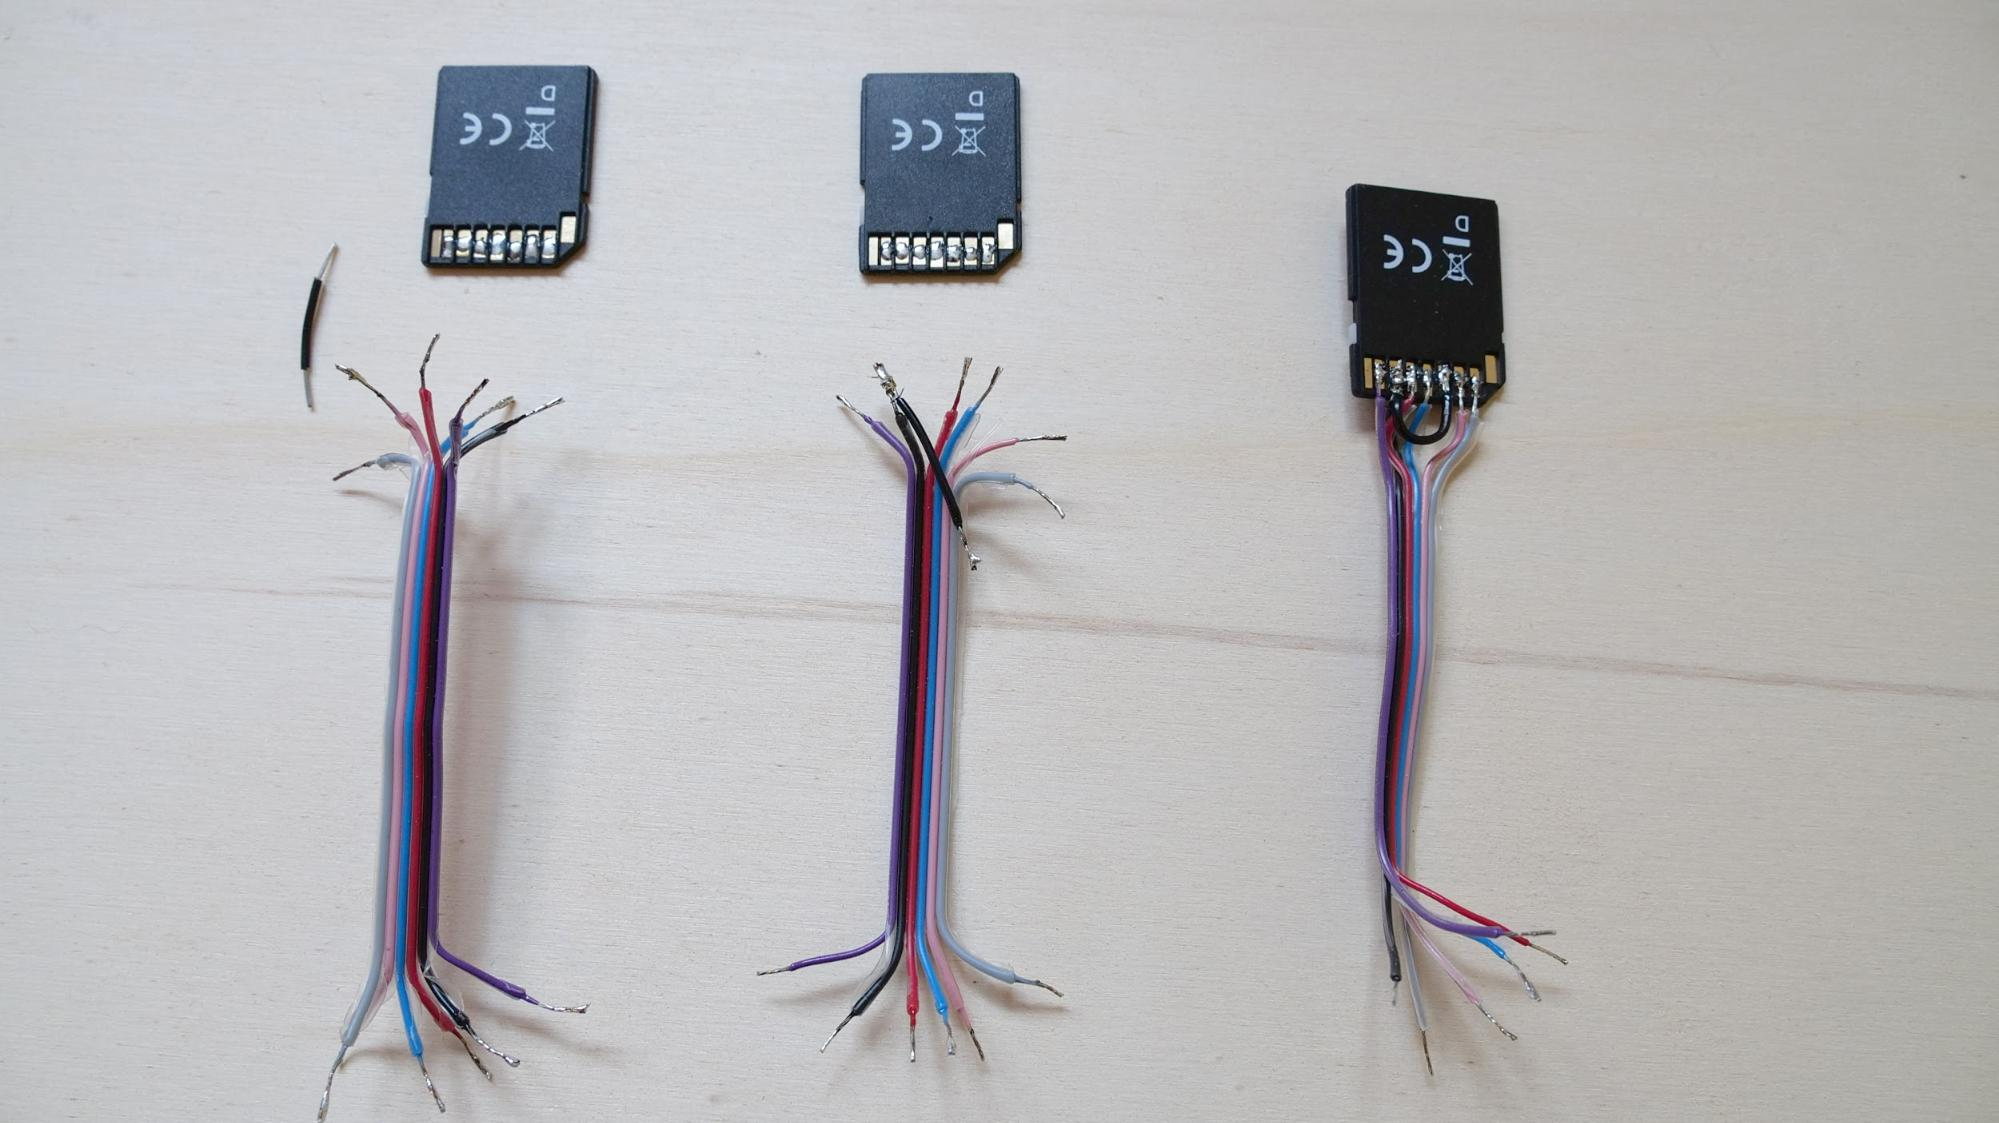
\includegraphics{images/image4.jpg}}

{Die SD-Karte wird fast wie in diesem Beispiel angeschlossen:}

{\href{https://www.google.com/url?q=https://camo.githubusercontent.com/fe6b89251ae4df2628b1a4c86c57976f22d6d5ba/687474703a2f2f692e696d6775722e636f6d2f34436f584f75522e706e67\&sa=D\&ust=1588976963798000}{https://camo.githubusercontent.com/fe6b89251ae4df2628b1a4c86c57976f22d6d5ba/687474703a2f2f692e696d6775722e636f6d2f34436f584f75522e706e67}}

{}

{Nur VCC und GND werden nicht direkt am ESP32 angeschlossen.}

{}

\protect\hypertarget{t.dfc647e596c2e4387a04c10c877e17b08bda1dd3}{}{}\protect\hypertarget{t.1}{}{}

\begin{longtable}[]{@{}lll@{}}
\toprule
\endhead
{Bezeichnung} & {Farbe} & {ESP32 Pin}\tabularnewline
{MISO} & {Lila} & {19}\tabularnewline
{GND} & {Schwarz} & {}\tabularnewline
{CLK} & {Rot} & {18}\tabularnewline
{VCC} & {Blau} & {}\tabularnewline
{GND} & {Schwarz} & {}\tabularnewline
{MOSI} & {Rosa} & {23}\tabularnewline
{CS} & {Grau} & {5}\tabularnewline
\bottomrule
\end{longtable}

\begin{center}\rule{0.5\linewidth}{0.5pt}\end{center}

{}

{}

\begin{enumerate}
\setcounter{enumi}{1}
\tightlist
\item
  {GPS-Modul}
\end{enumerate}

{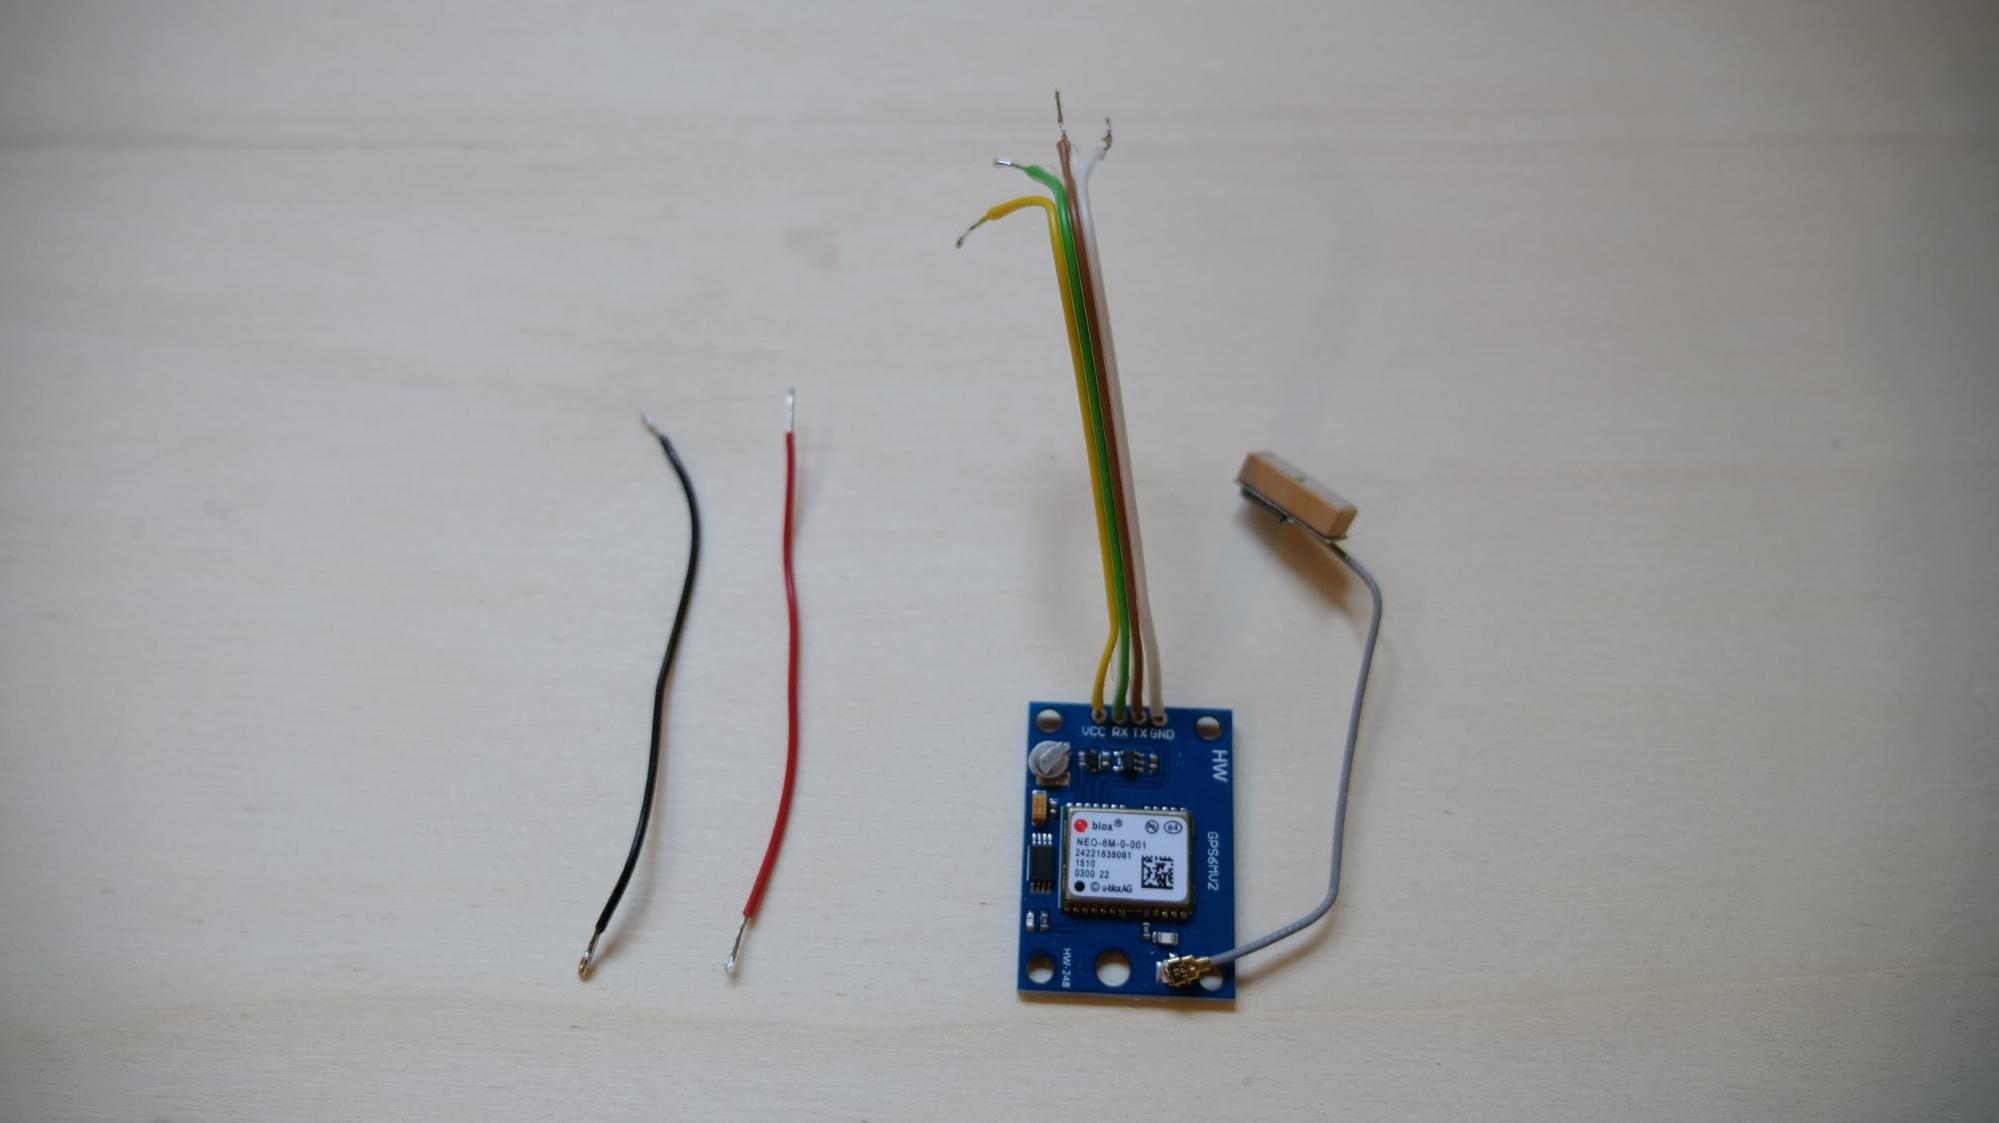
\includegraphics{images/image9.jpg}}

{}

{}

\protect\hypertarget{t.1f25748bf503468b1e7bbd2d76883e77108db989}{}{}\protect\hypertarget{t.2}{}{}

\begin{longtable}[]{@{}lll@{}}
\toprule
\endhead
{Bezeichnung} & {Farbe} & {ESP32 Pin}\tabularnewline
{VCC} & {Gelb} & {-\/-\/-}\tabularnewline
{RX} & {Grün} & {17}\tabularnewline
{TX} & {Braun} & {16}\tabularnewline
{GND} & {Weiß} & {-\/-\/-}\tabularnewline
\bottomrule
\end{longtable}

\begin{center}\rule{0.5\linewidth}{0.5pt}\end{center}

{}

{}

{}

{}

\begin{enumerate}
\setcounter{enumi}{2}
\tightlist
\item
  {Ultraschallsensoren}
\end{enumerate}

{}

\protect\hypertarget{t.5c49095038b0b1a505dffa0c95a0f90e5dde1431}{}{}\protect\hypertarget{t.3}{}{}

\begin{longtable}[]{@{}lll@{}}
\toprule
\endhead
{Sensor am Deckel} & {Farbe} & {ESP32 Pin}\tabularnewline
{VCC} & {Rot - kurze Brücke zu anderem Sensor} &
{-\/-\/-}\tabularnewline
{Trig} & {Grün} & {15}\tabularnewline
{Echo} & {Orange} & {4}\tabularnewline
{GND} & {Schwarz - kurze Brücke zu anderem Sensor} &
{-\/-\/-}\tabularnewline
\bottomrule
\end{longtable}

{}

{}

\protect\hypertarget{t.c88803b3ec9656d93950427e71cffac21c21c201}{}{}\protect\hypertarget{t.4}{}{}

\begin{longtable}[]{@{}lll@{}}
\toprule
\endhead
{Sensor im Gehäuse} & {Farbe} & {ESP32 Pin}\tabularnewline
{VCC} & {Rot} & {-\/-\/-}\tabularnewline
{Trig} & {Grün} & {25}\tabularnewline
{Echo} & {Orange} & {26}\tabularnewline
{GND} & {Schwarz} & {-\/-\/-}\tabularnewline
\bottomrule
\end{longtable}

{}

\begin{center}\rule{0.5\linewidth}{0.5pt}\end{center}

{}

\begin{enumerate}
\setcounter{enumi}{3}
\tightlist
\item
  {Stecker zum Display}
\end{enumerate}

{}

\protect\hypertarget{t.7615705d67f555cade8b8088d668b61e9c94ee1e}{}{}\protect\hypertarget{t.5}{}{}

\begin{longtable}[]{@{}lll@{}}
\toprule
\endhead
{Bezeichnung} & {Stecker Pin} & {ESP32 Pin}\tabularnewline
{VCC} & {1} & {-\/-\/-}\tabularnewline
{SCL} & {2} & {22}\tabularnewline
{Druckknopf} & {3} & {2}\tabularnewline
{GND} & {4} & {-\/-\/-}\tabularnewline
{SDA} & {5} & {21}\tabularnewline
\bottomrule
\end{longtable}

{}

{}

{Druckknopf und Display teilen sich VCC. Der Pin am ESP32, an dem der Schalter hängt wird auch mit 10kOhm-Widerstand mit GND verbunden.}

{}

{}

{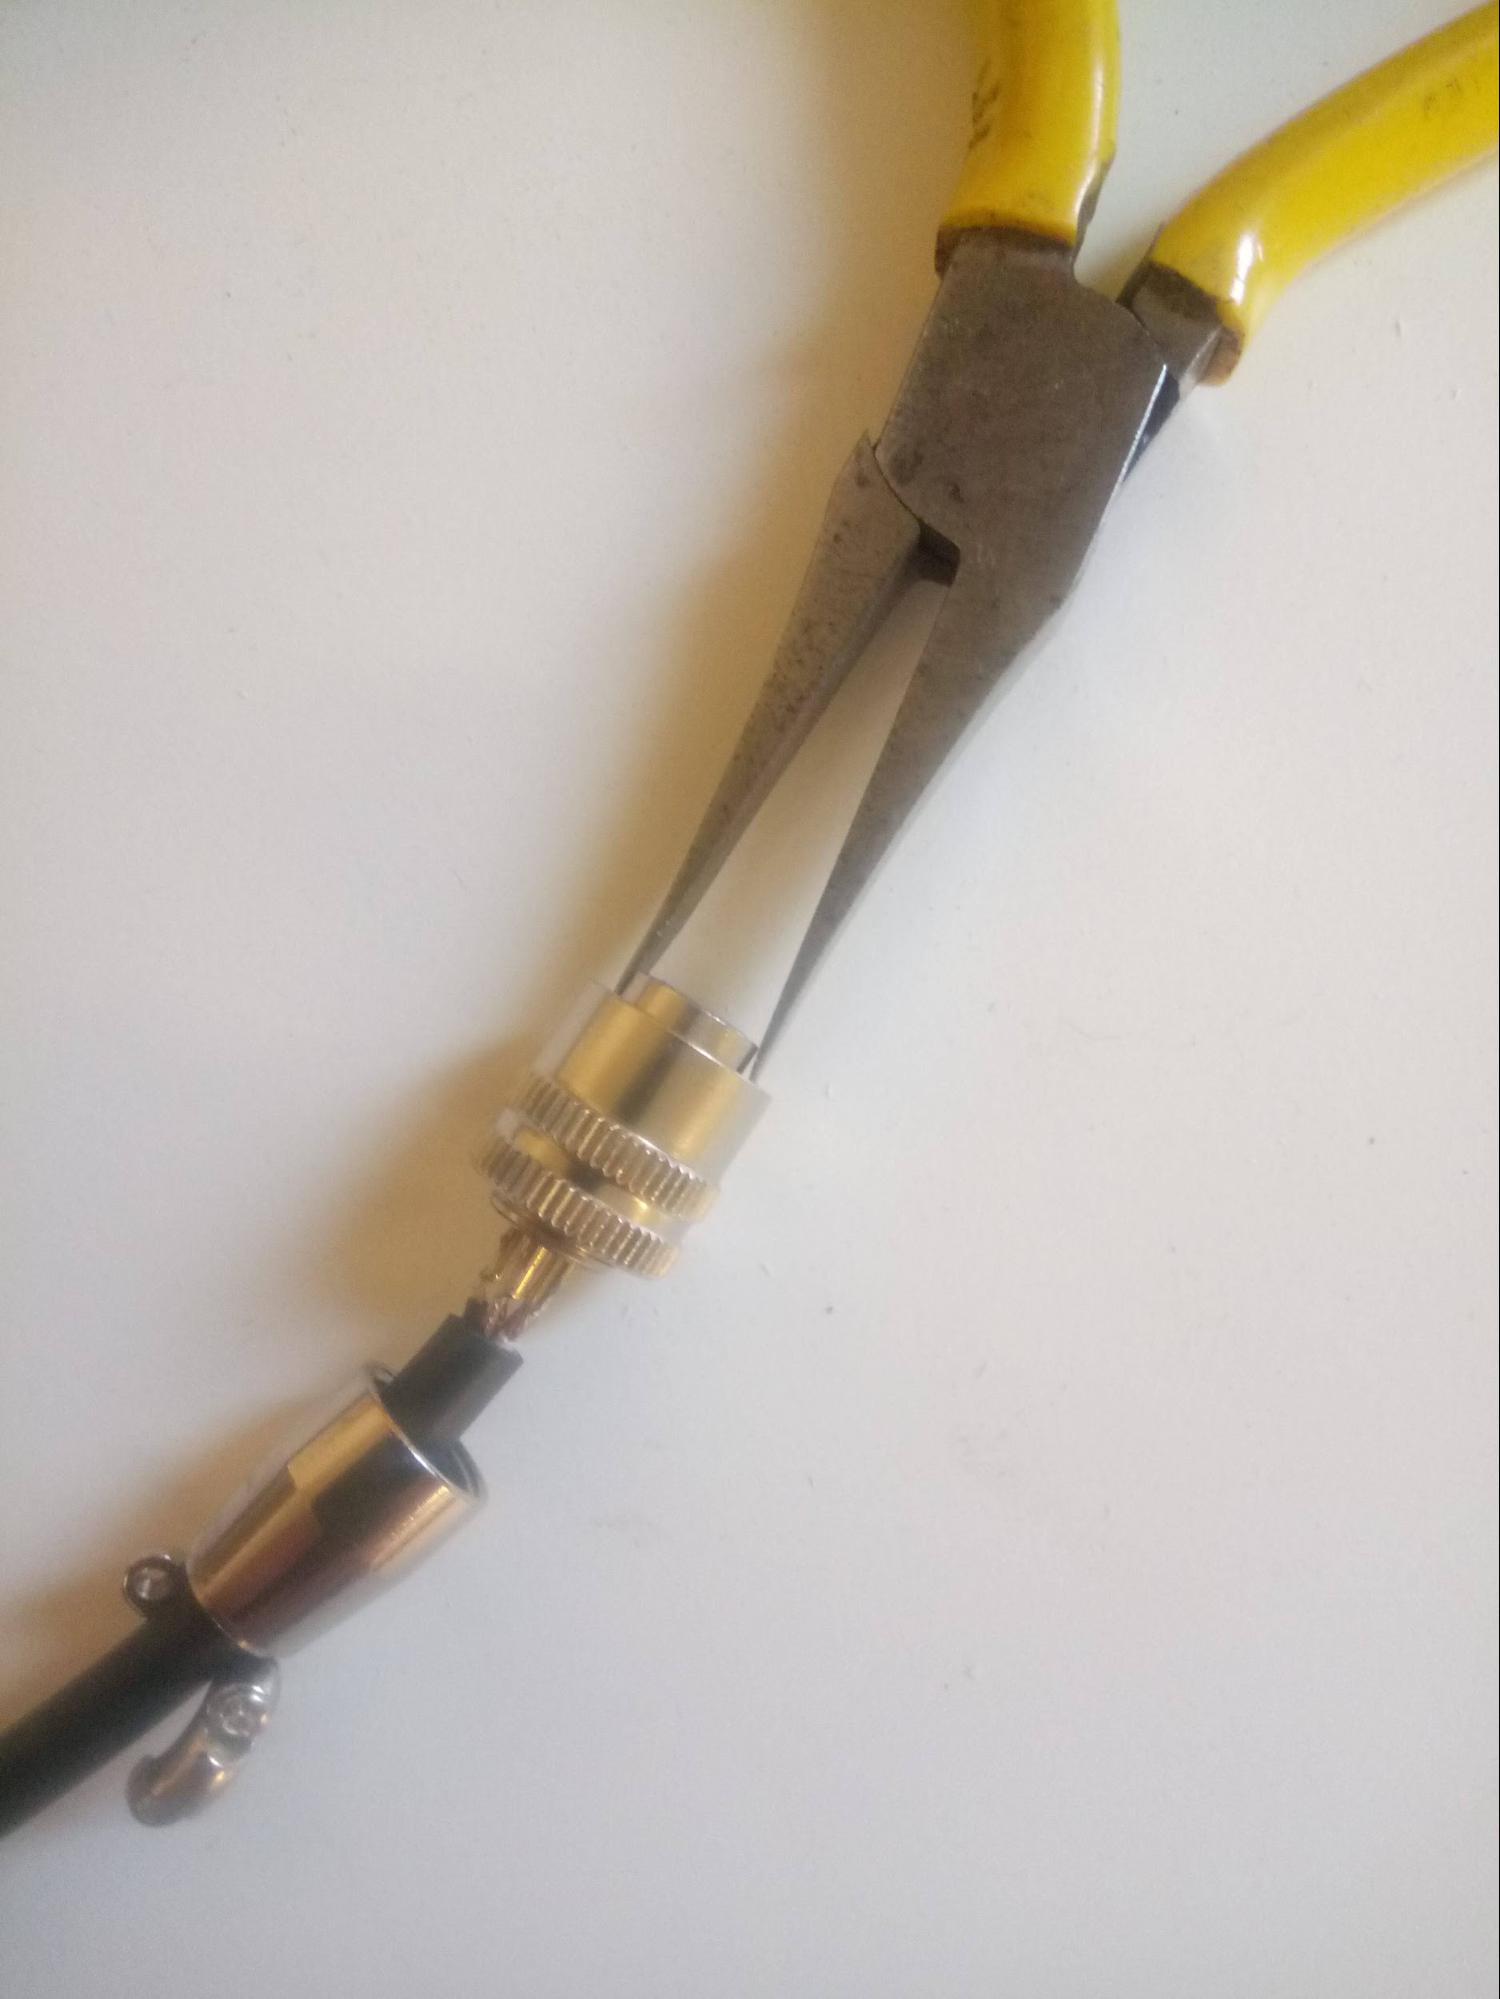
\includegraphics{images/image3.jpg}}

{}

{Die Kappe des Steckers ist raus zu schrauben. Die Außenisolierung des
Kabels sollte nur sehr knapp entfernt werden um die Zugentlastung
nachträglich fest schrauben zu können. (Zange zum Gegenhalten nur zur
Verdeutlichung, besser verwendet man den eingesteckten Stecker als
Gegenhalt.)}

\begin{center}\rule{0.5\linewidth}{0.5pt}\end{center}

{}

{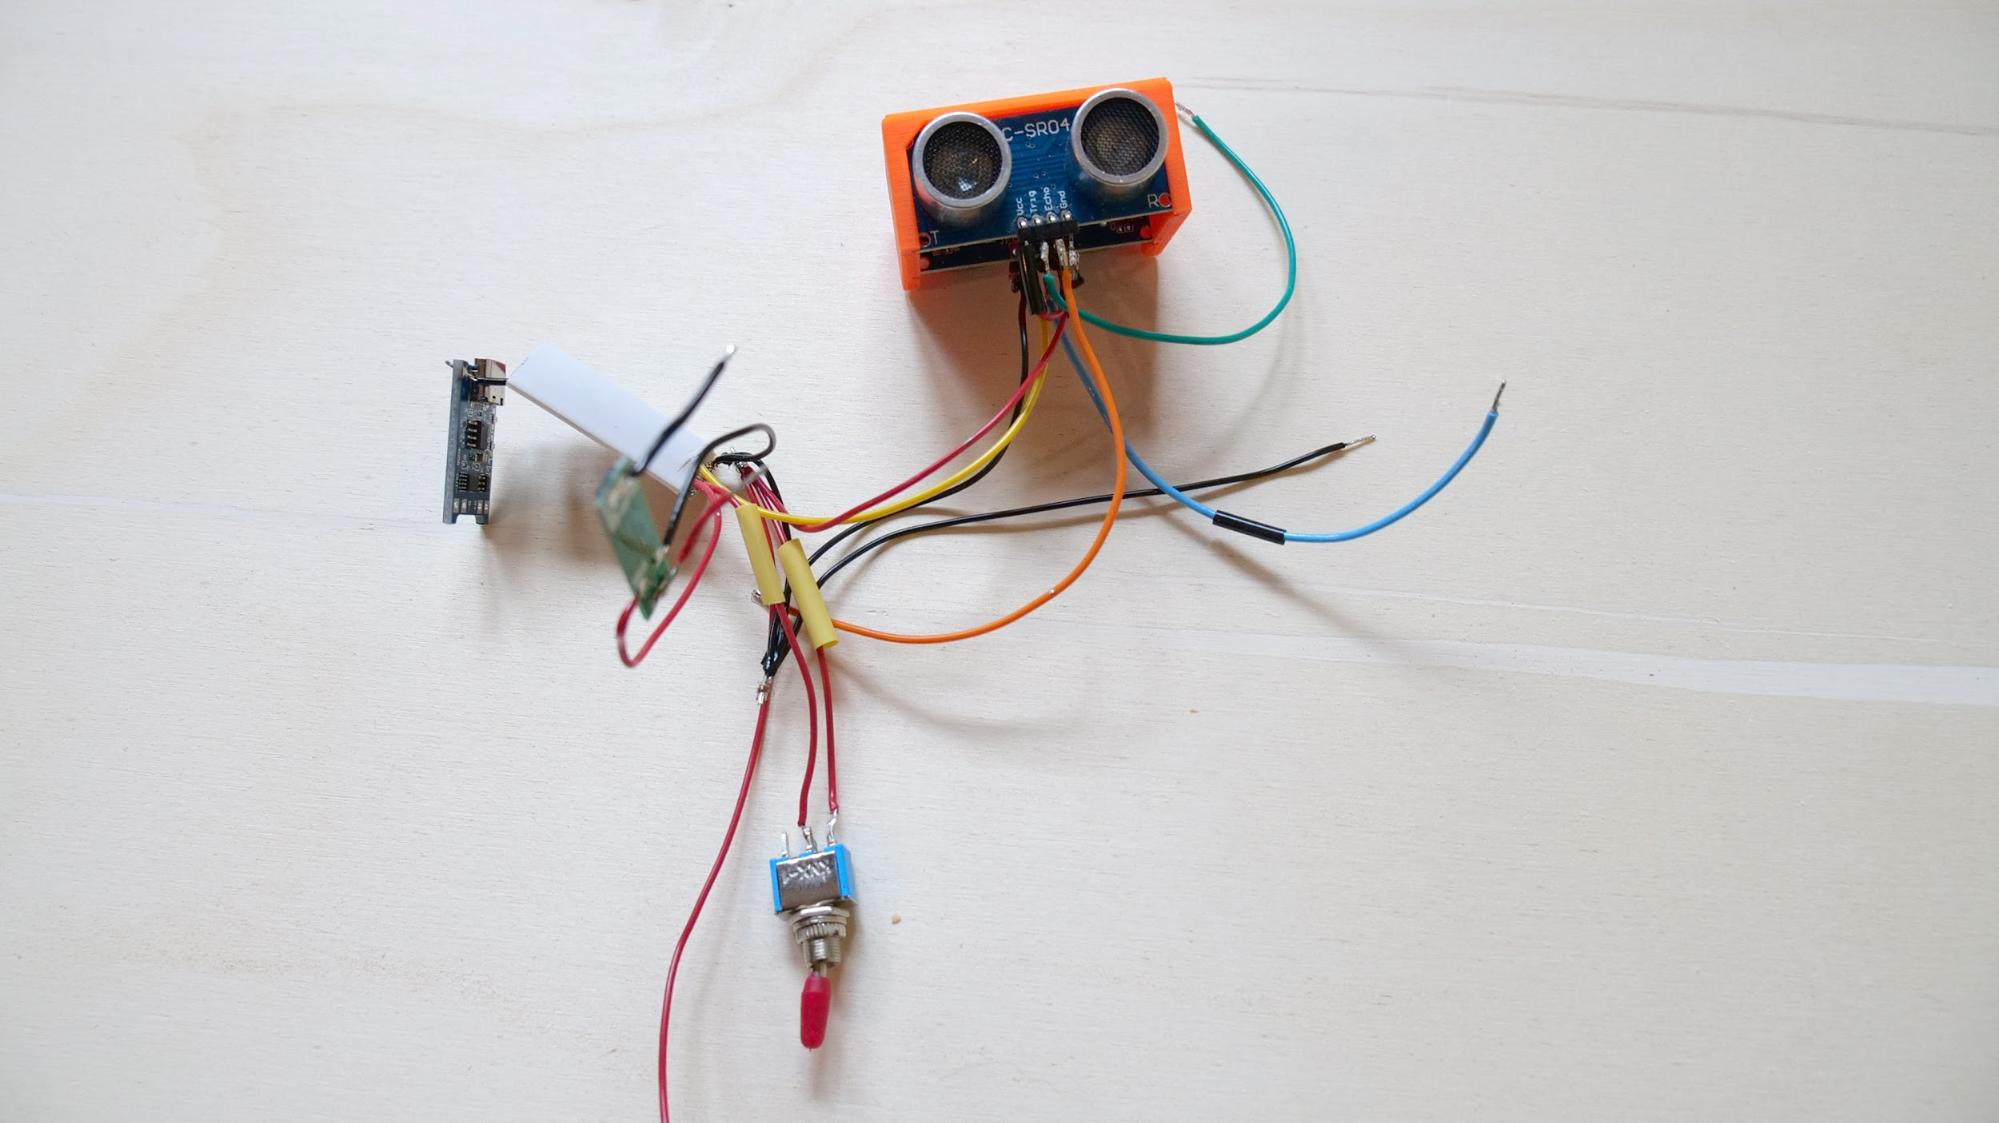
\includegraphics{images/image14.jpg}}

{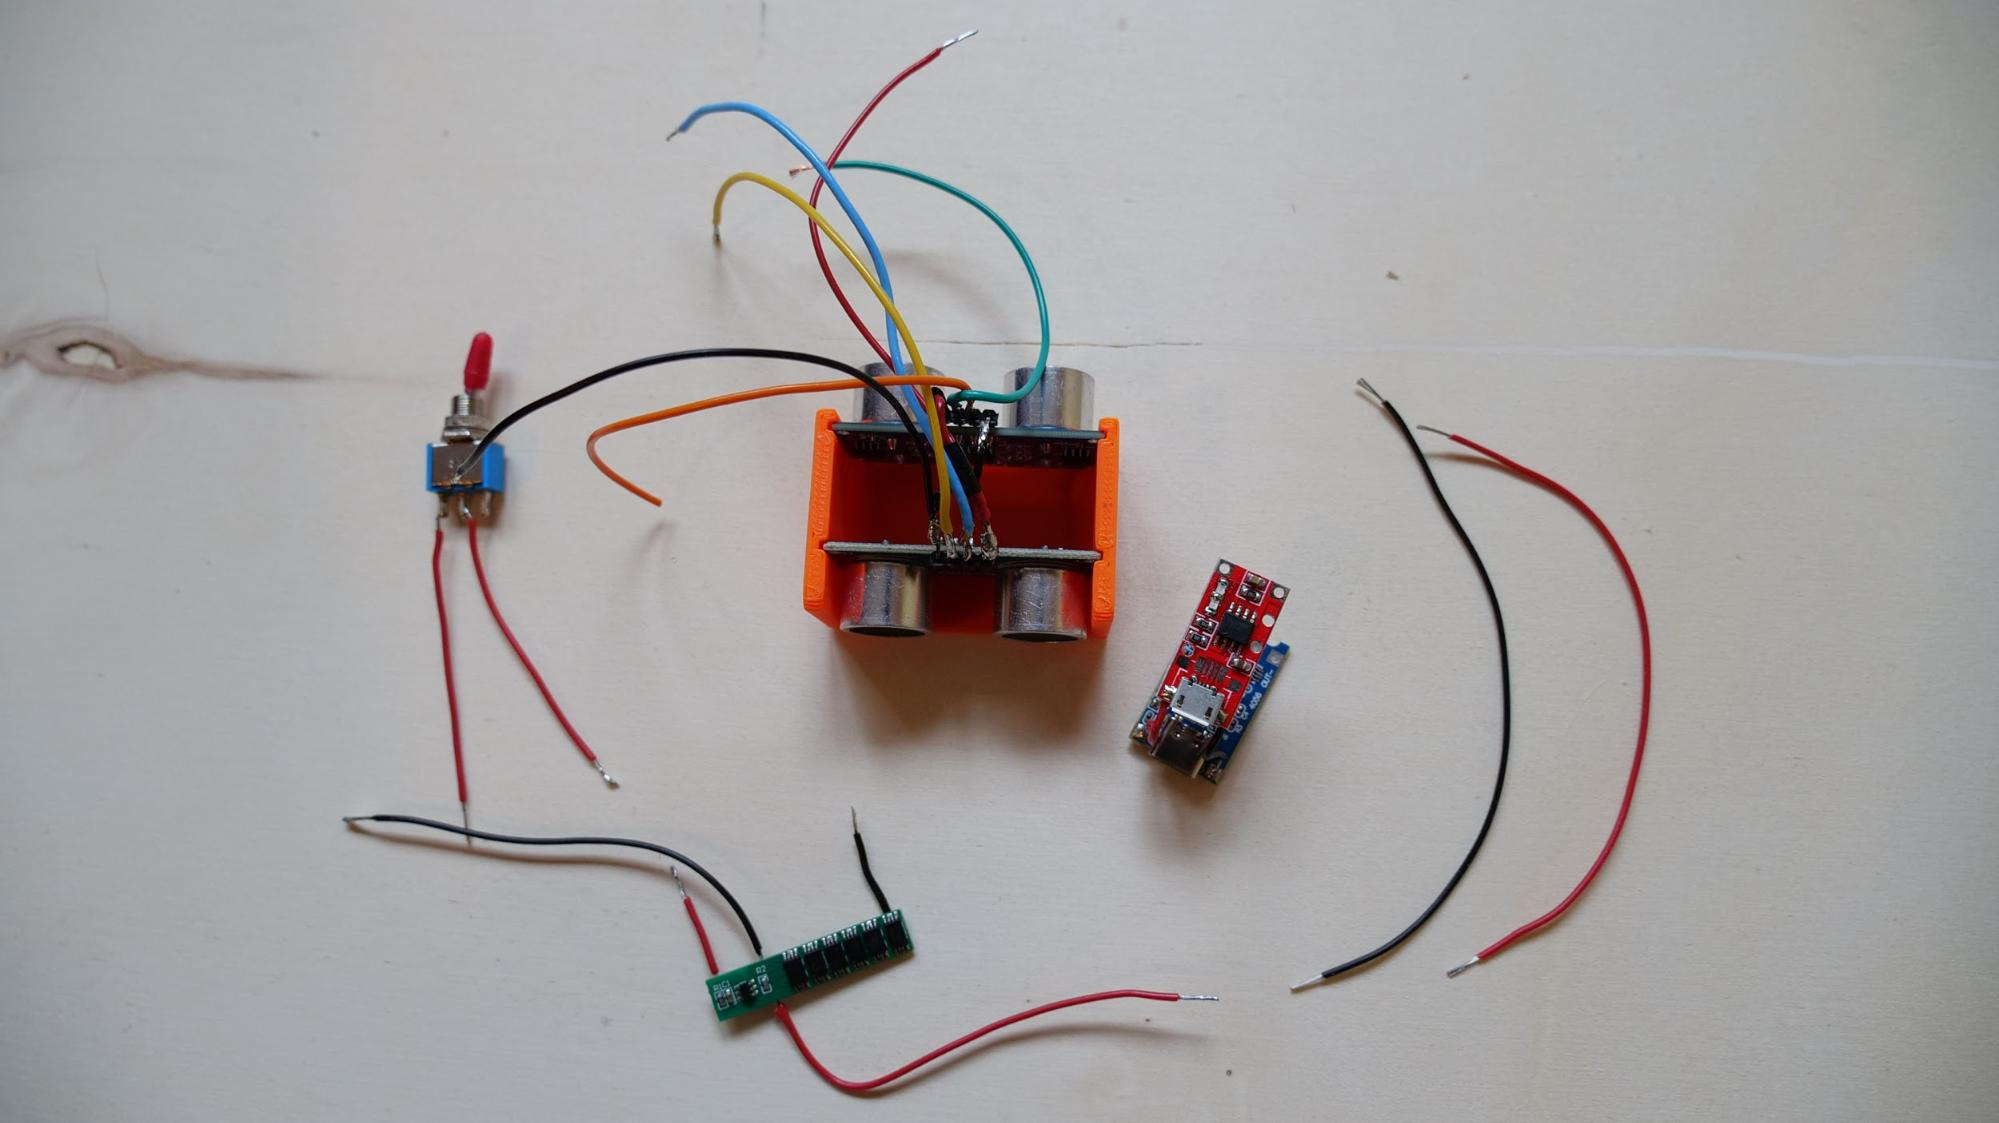
\includegraphics{images/image20.jpg}}

{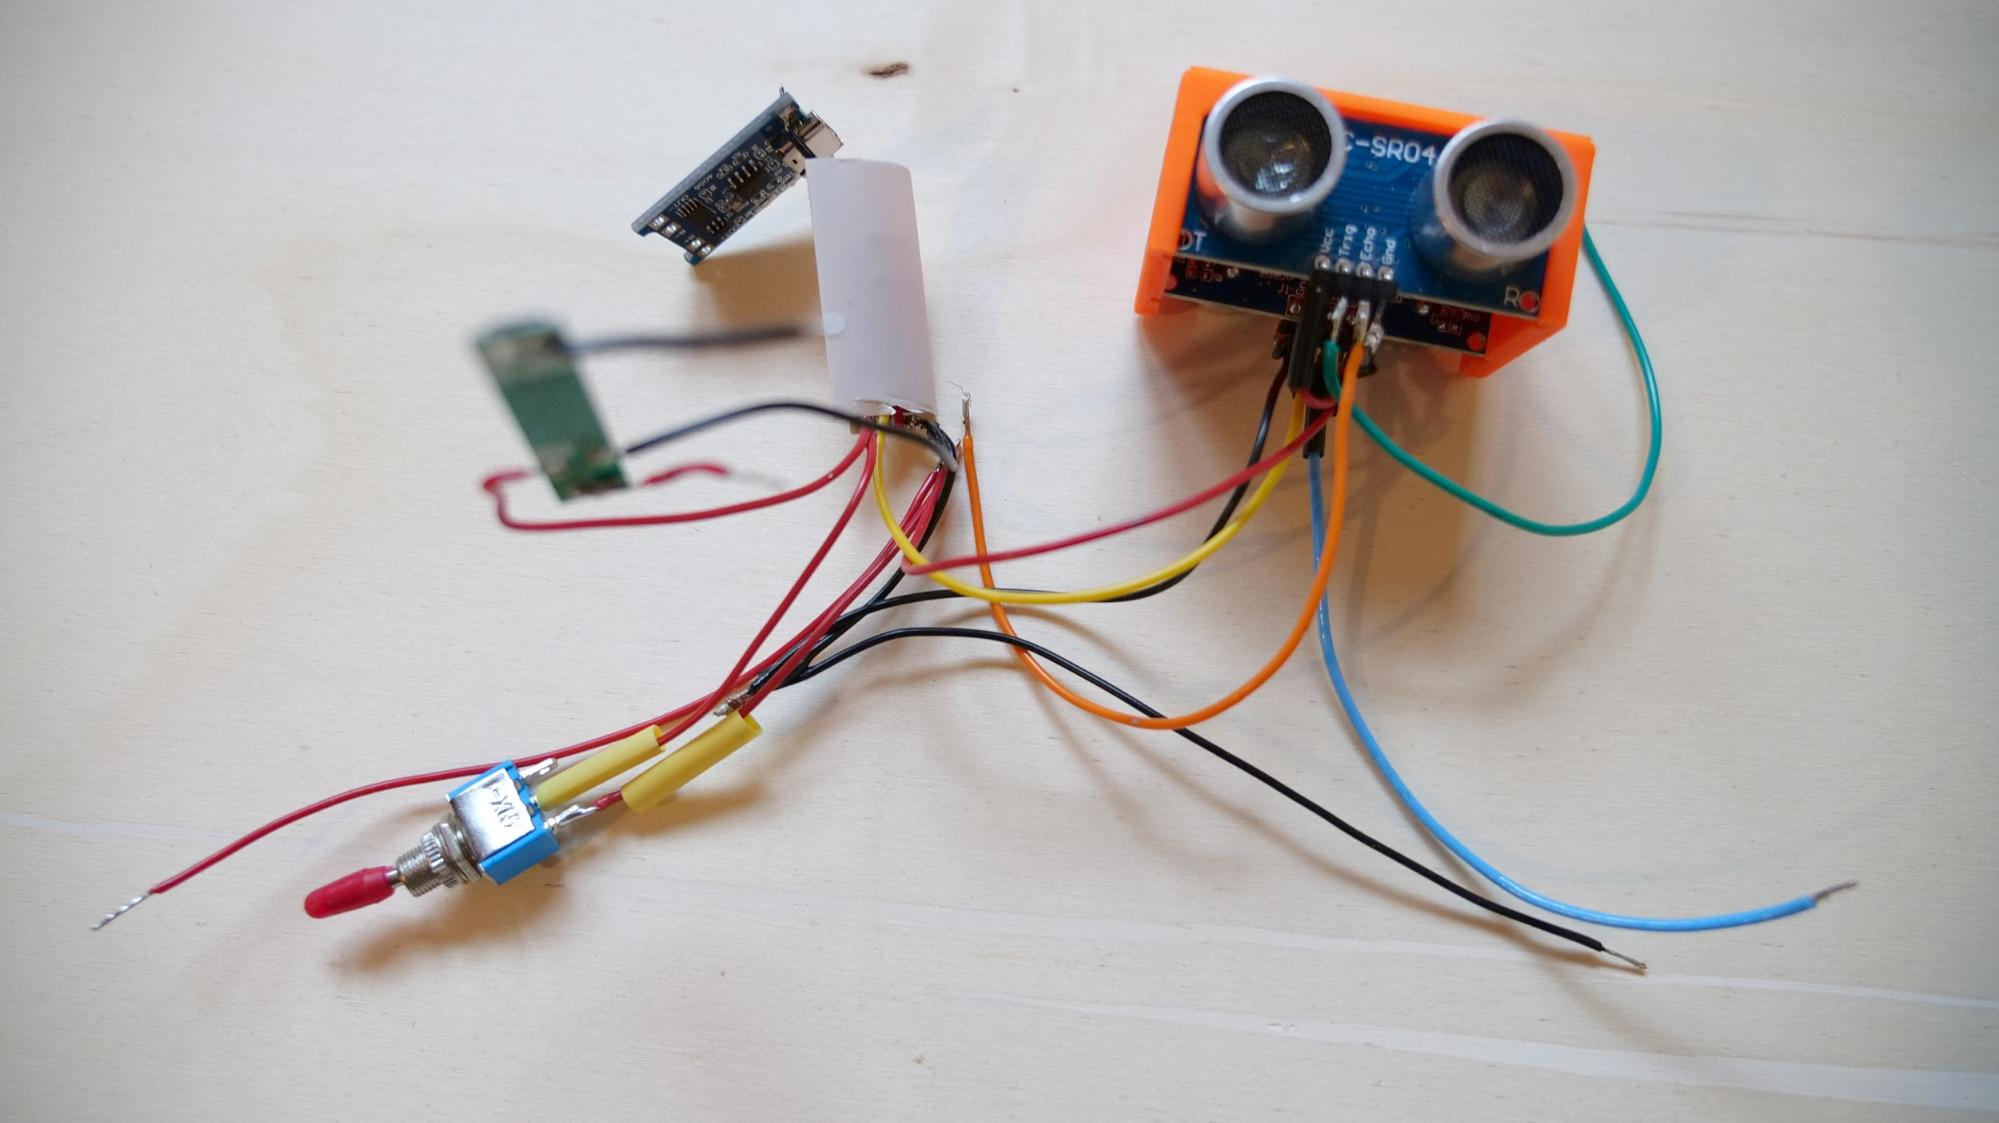
\includegraphics{images/image8.jpg}}

{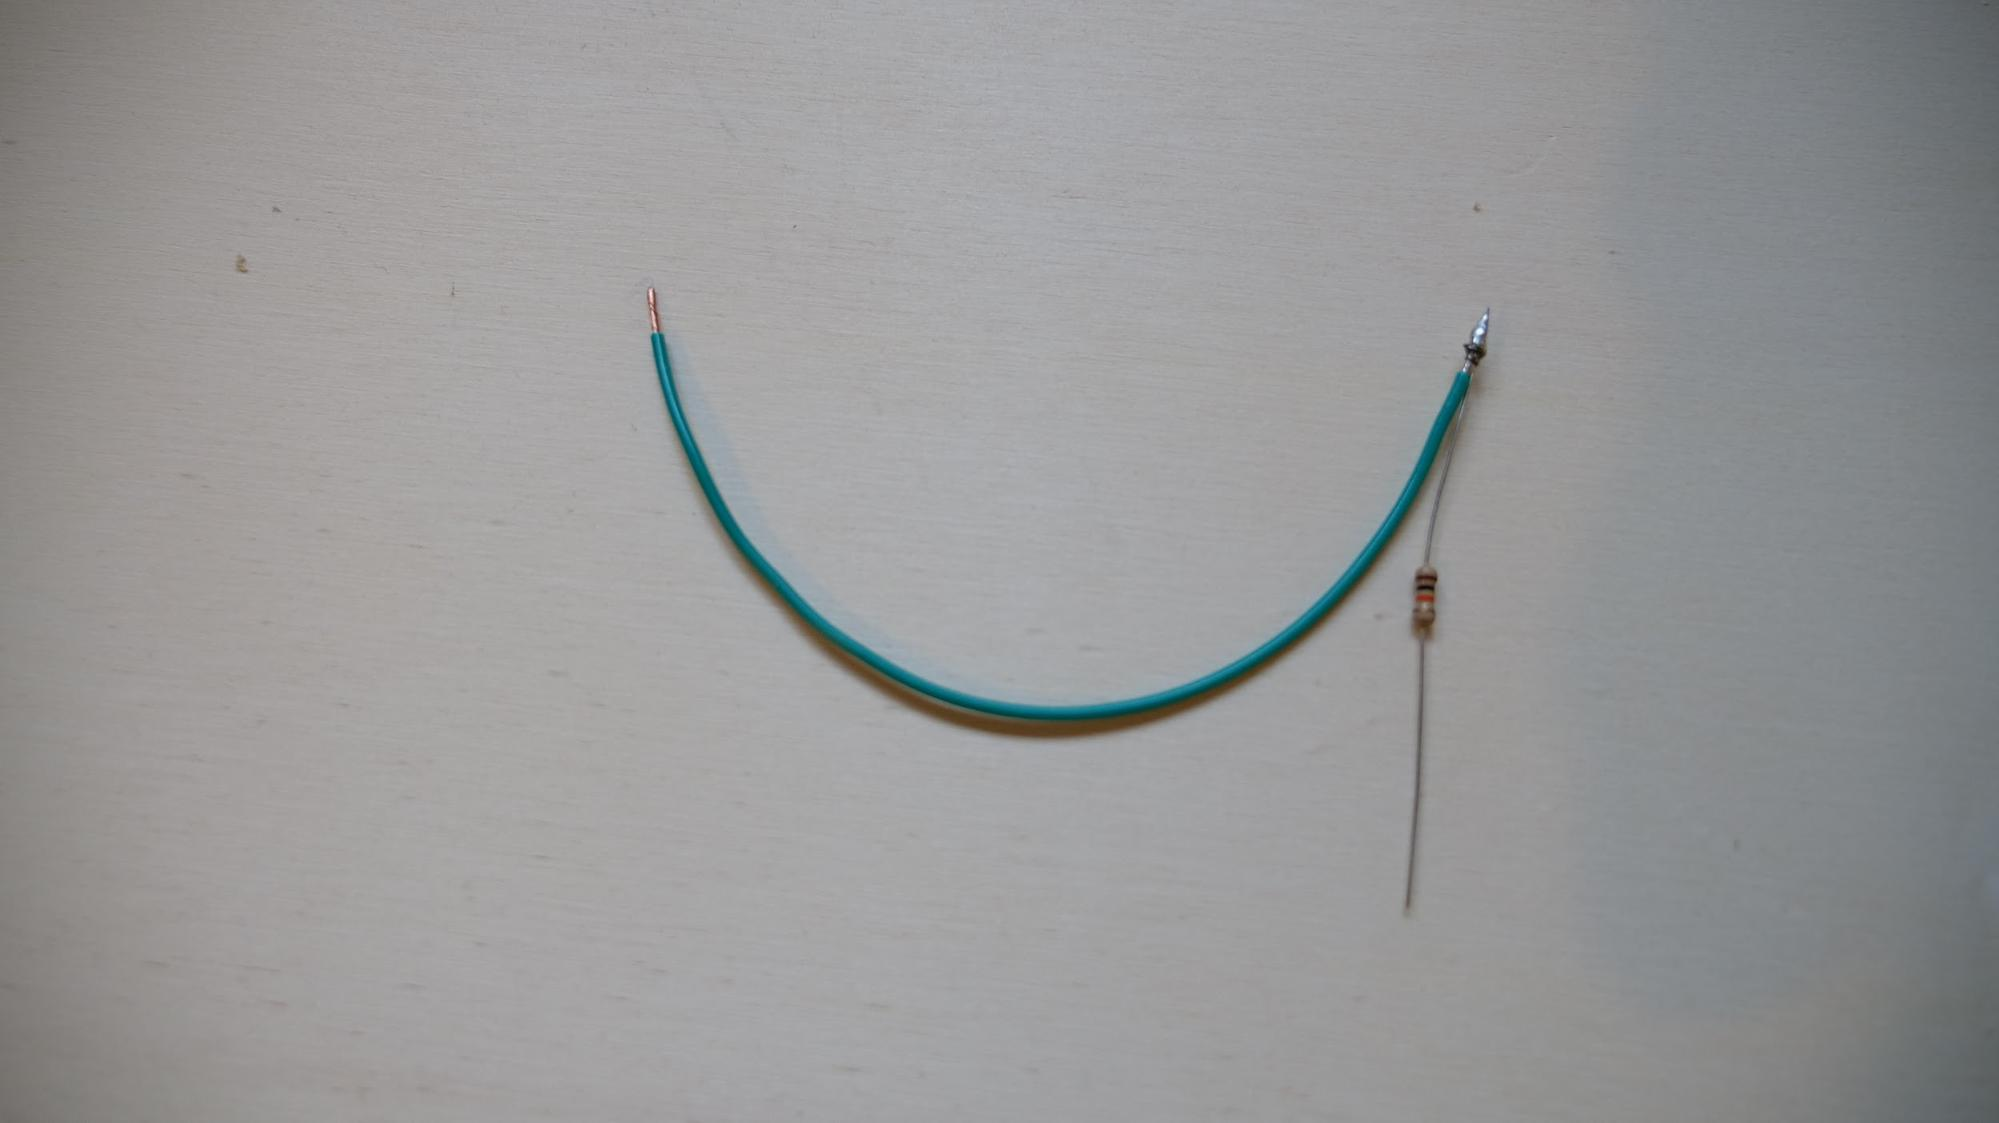
\includegraphics{images/image16.jpg}}

{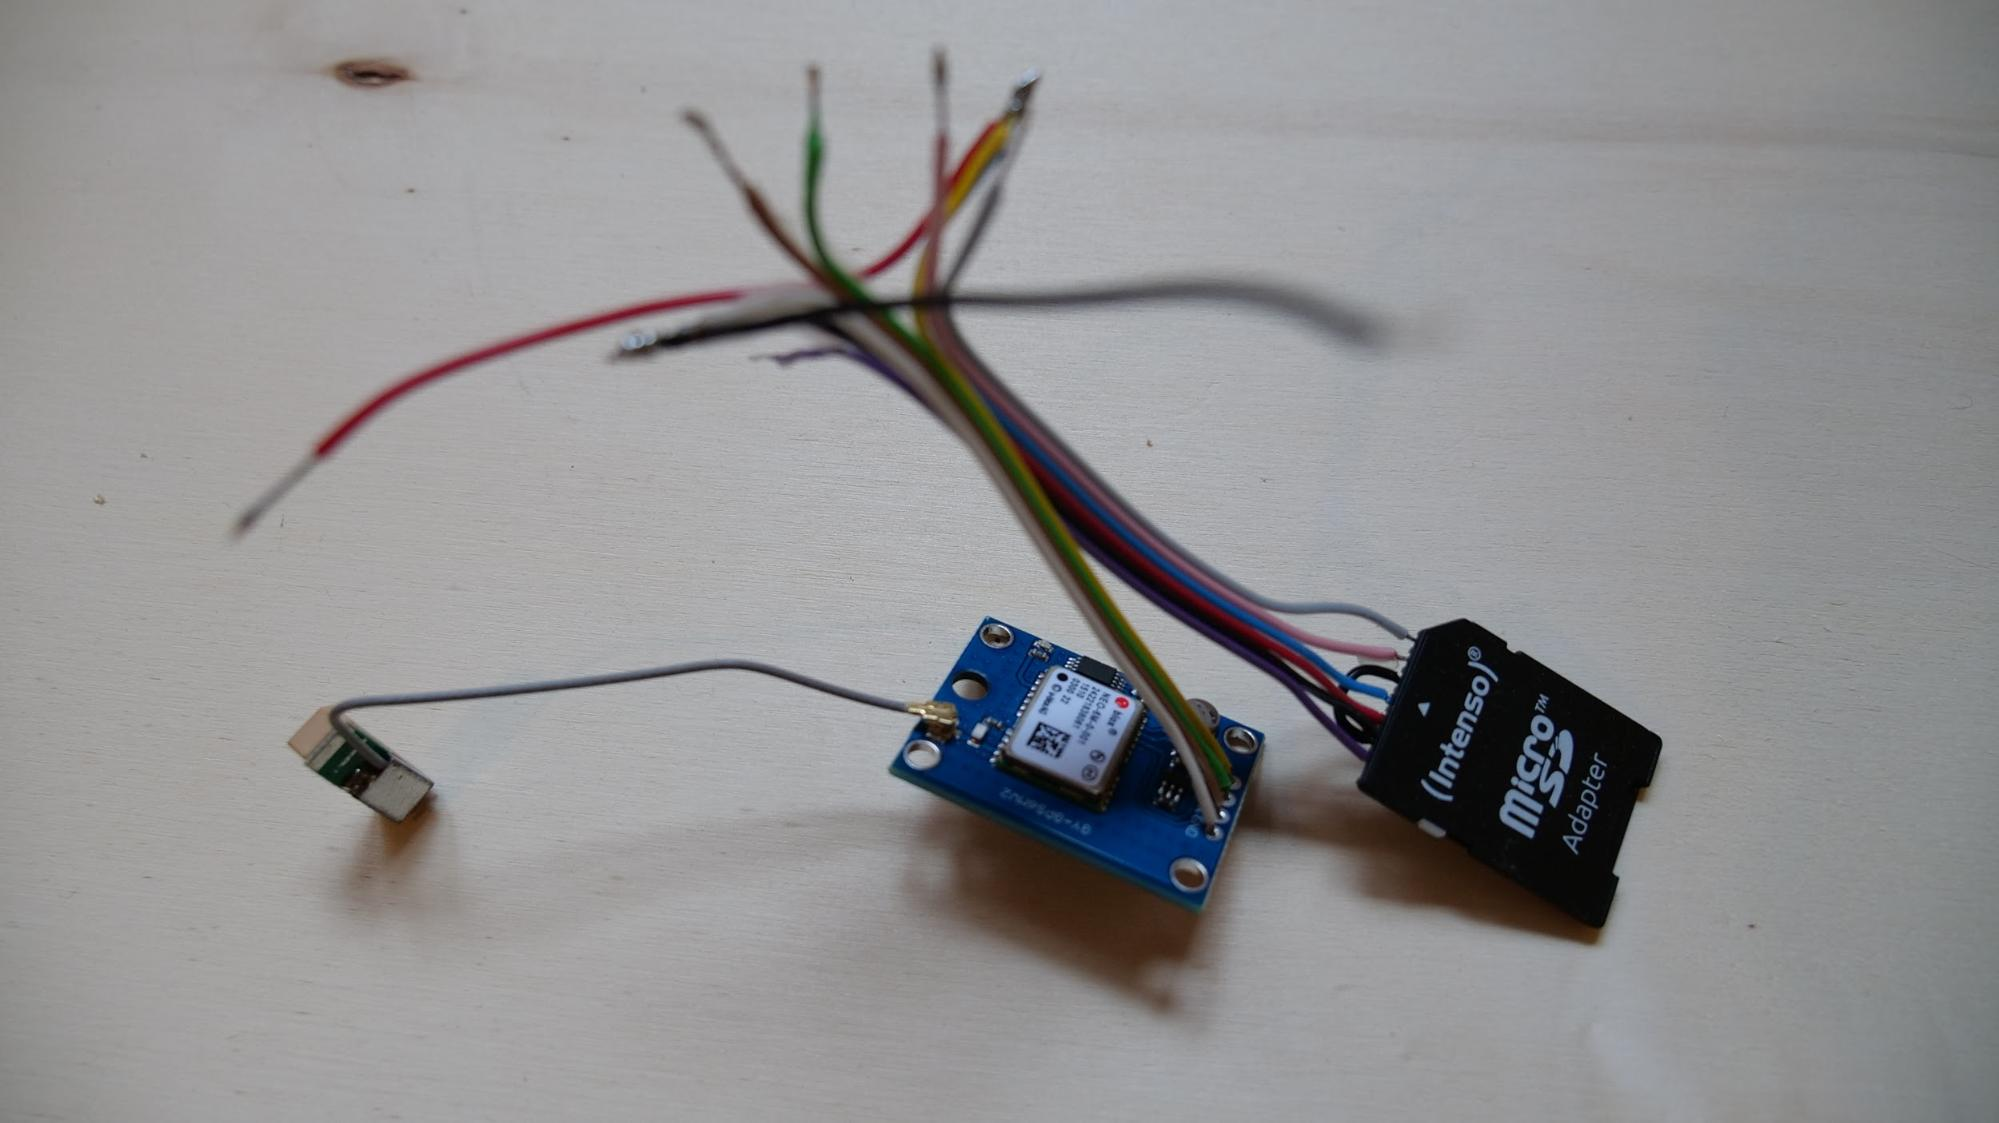
\includegraphics{images/image18.jpg}}

{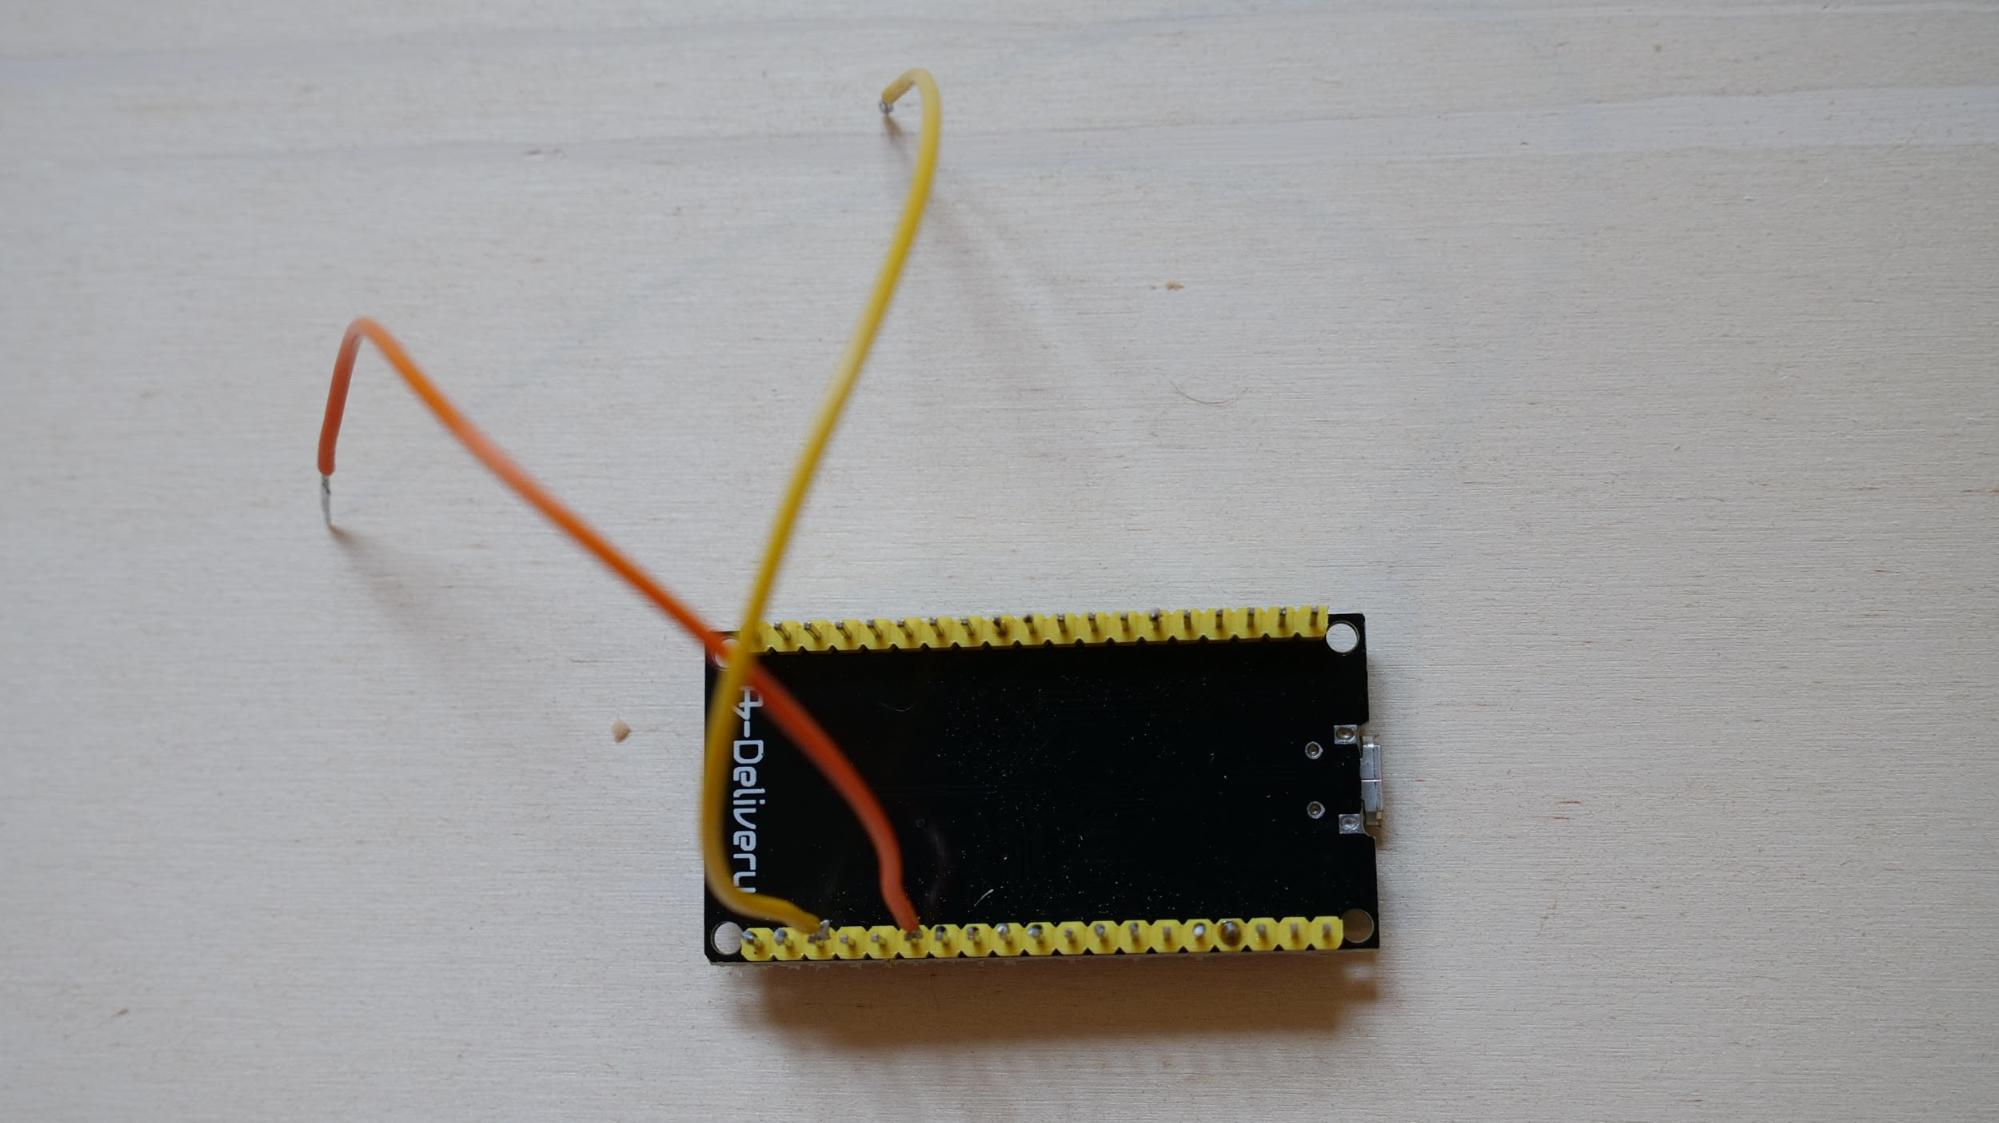
\includegraphics{images/image1.jpg}}

{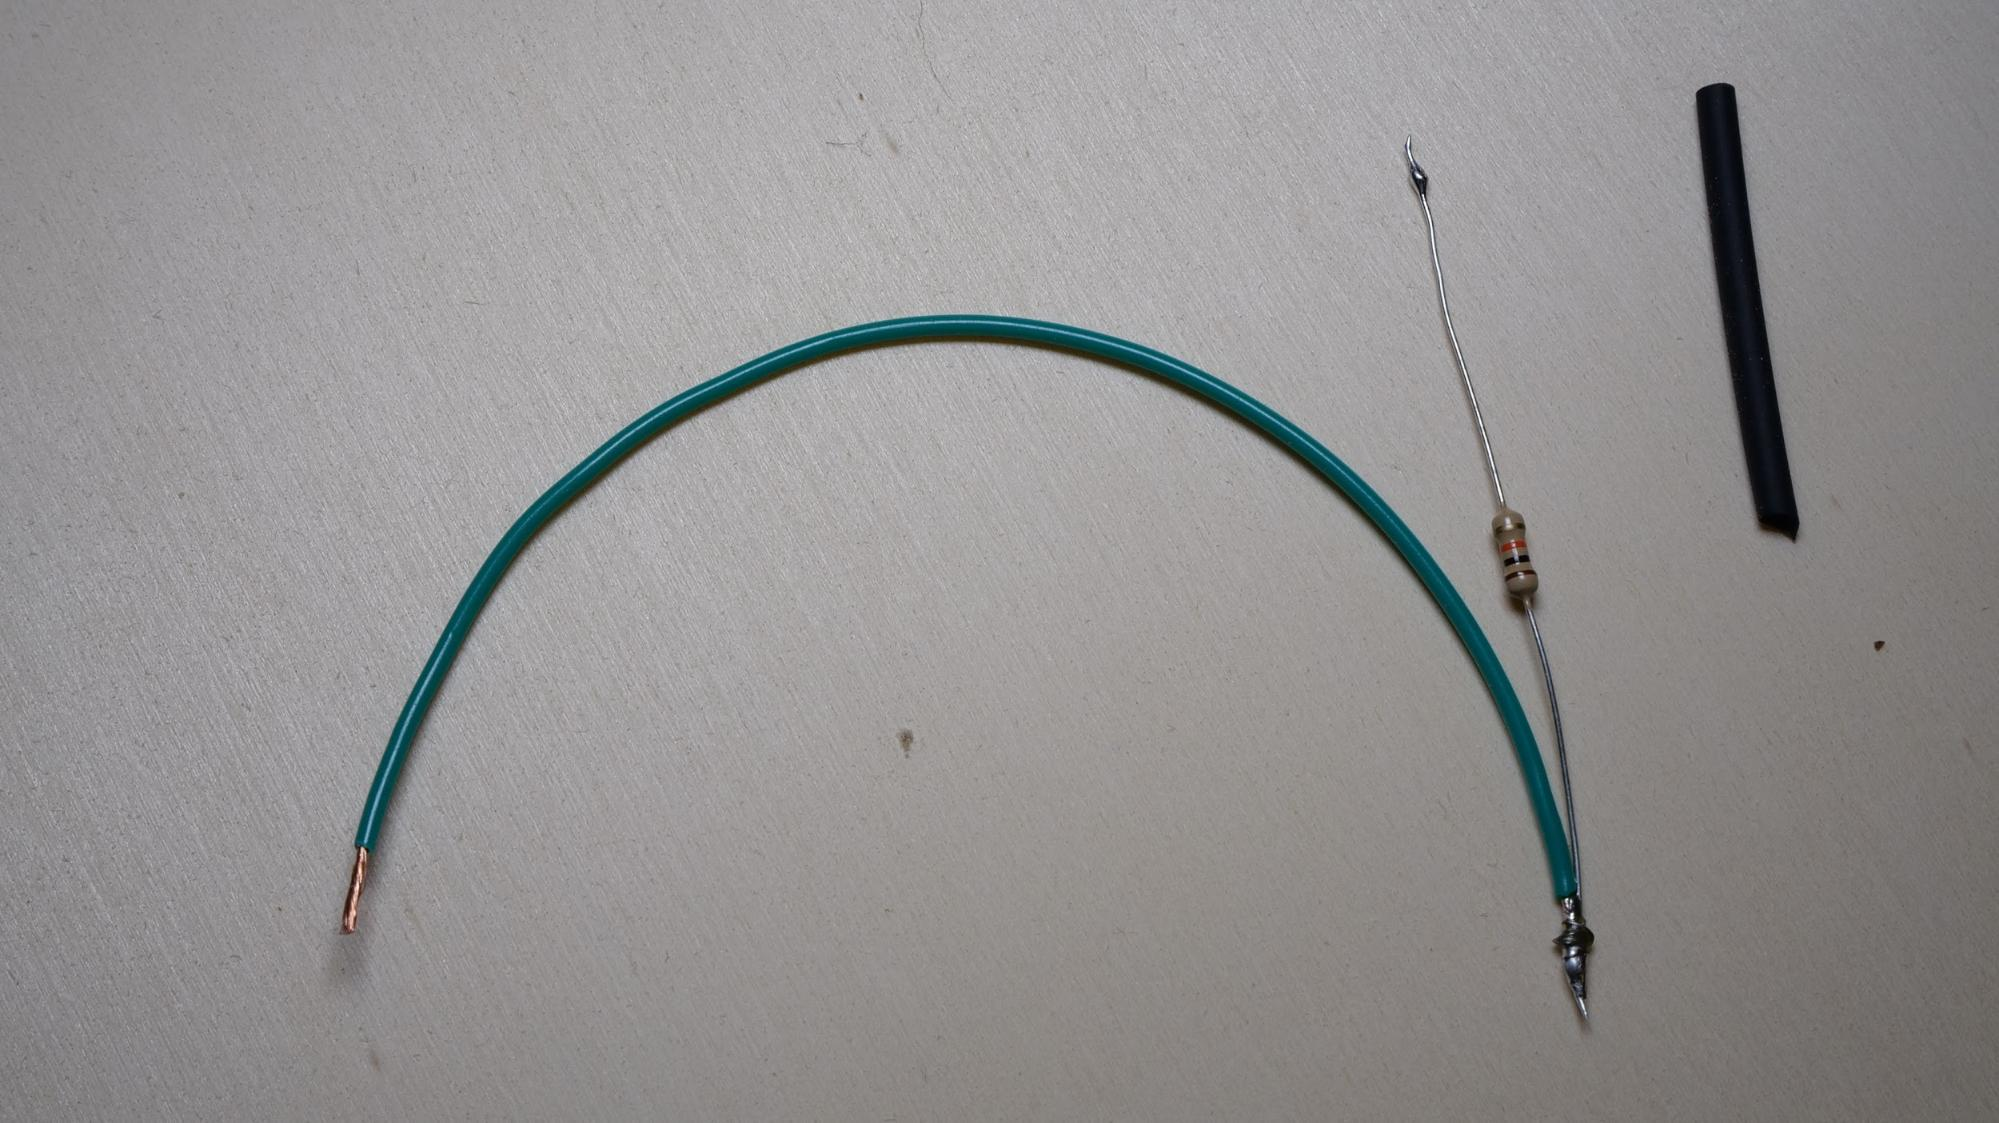
\includegraphics{images/image5.jpg}}

{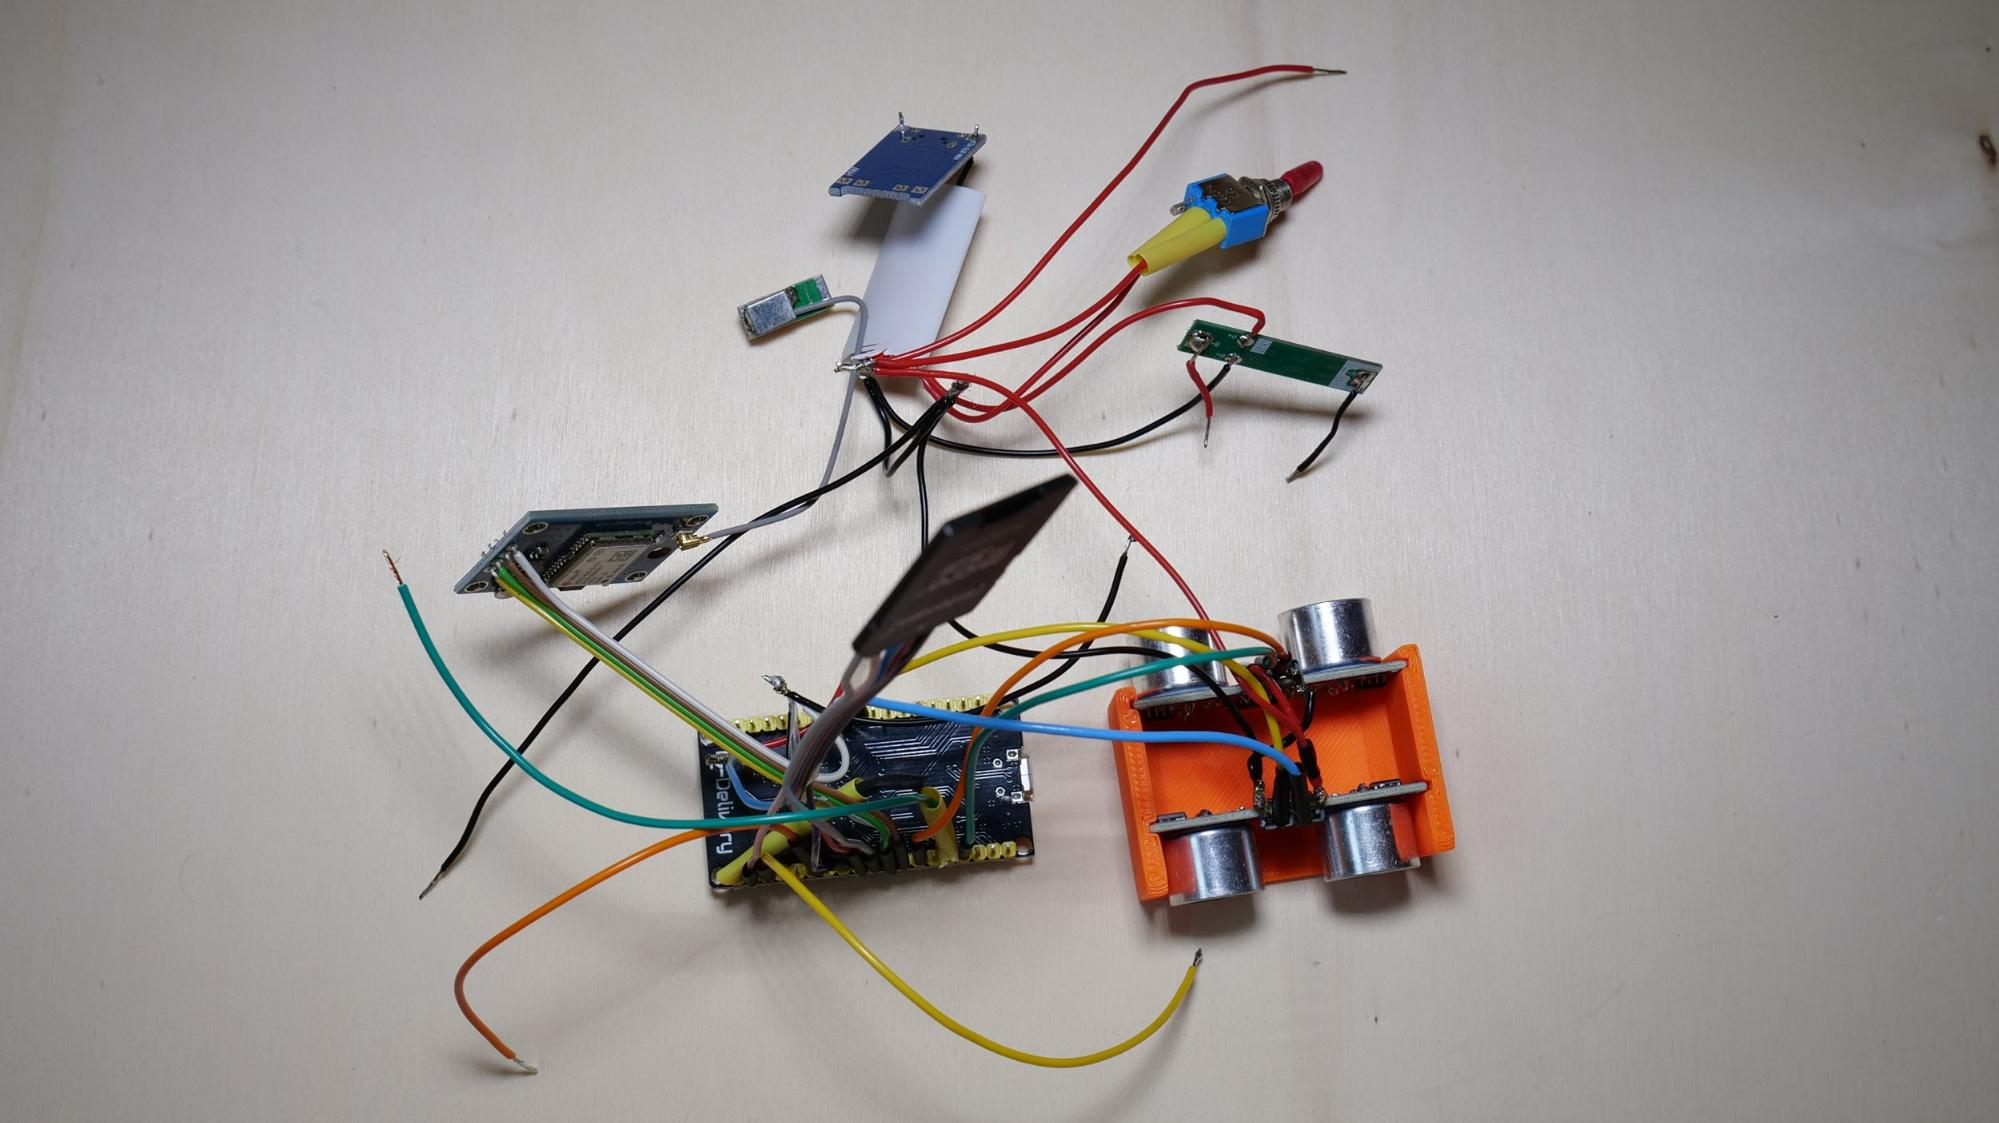
\includegraphics{images/image19.jpg}}

{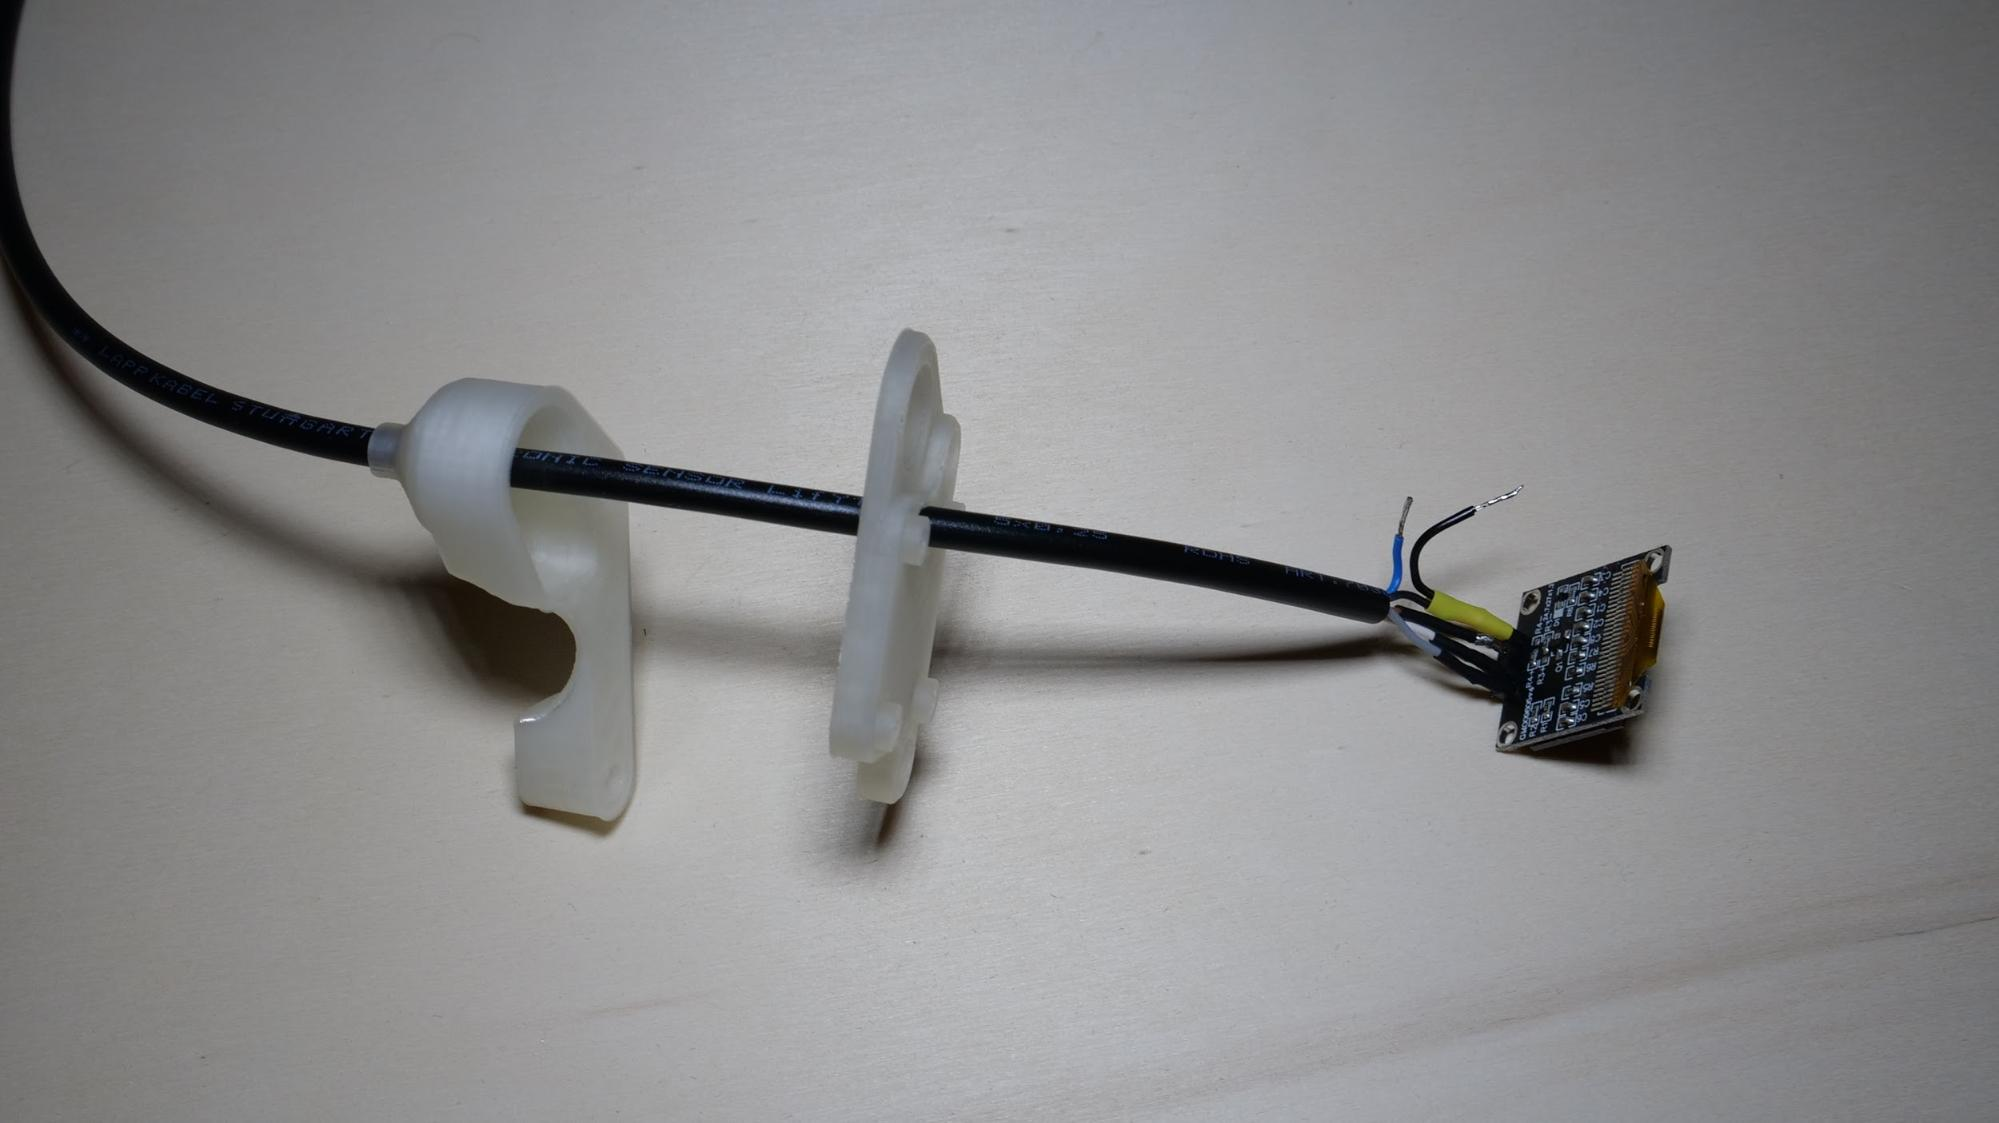
\includegraphics{images/image6.jpg}}

{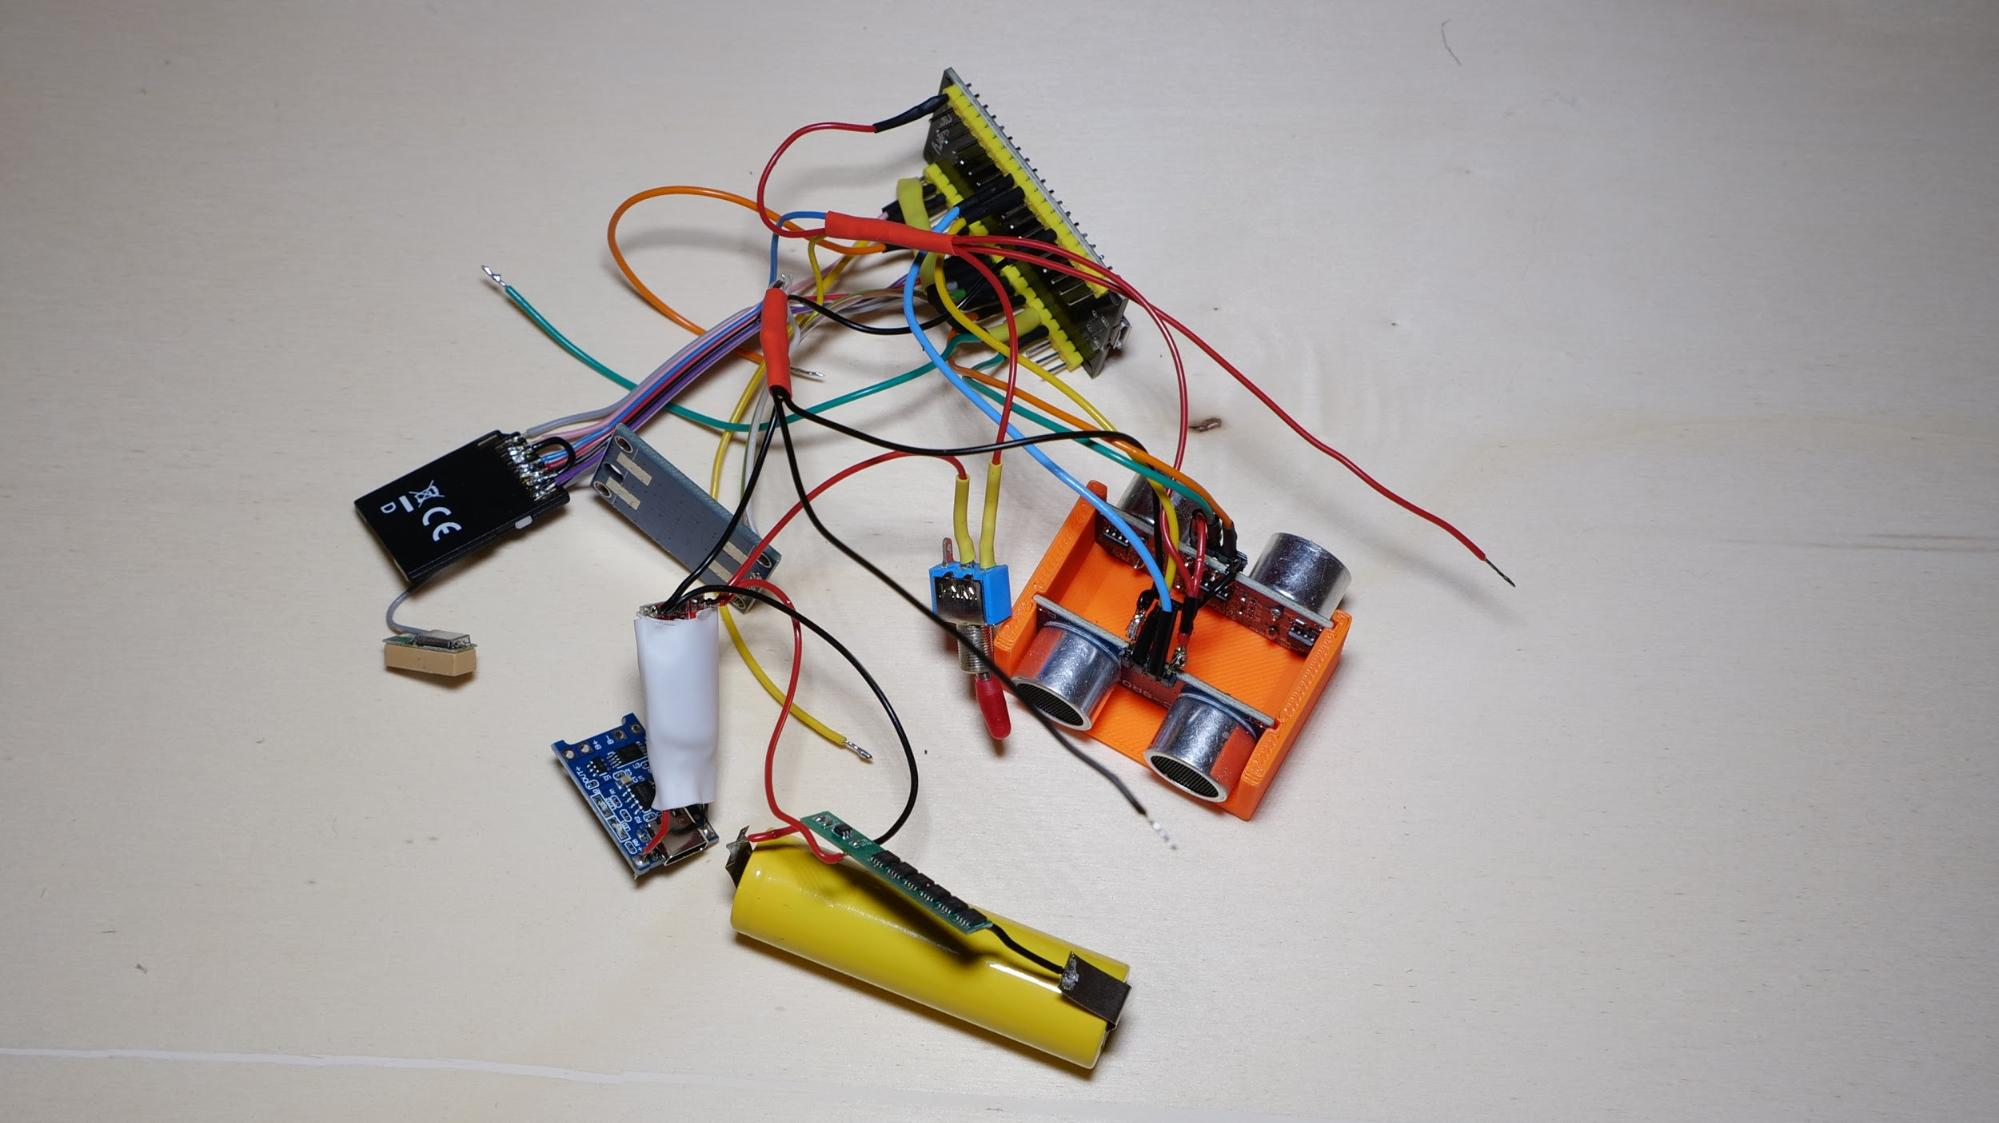
\includegraphics{images/image21.jpg}}

{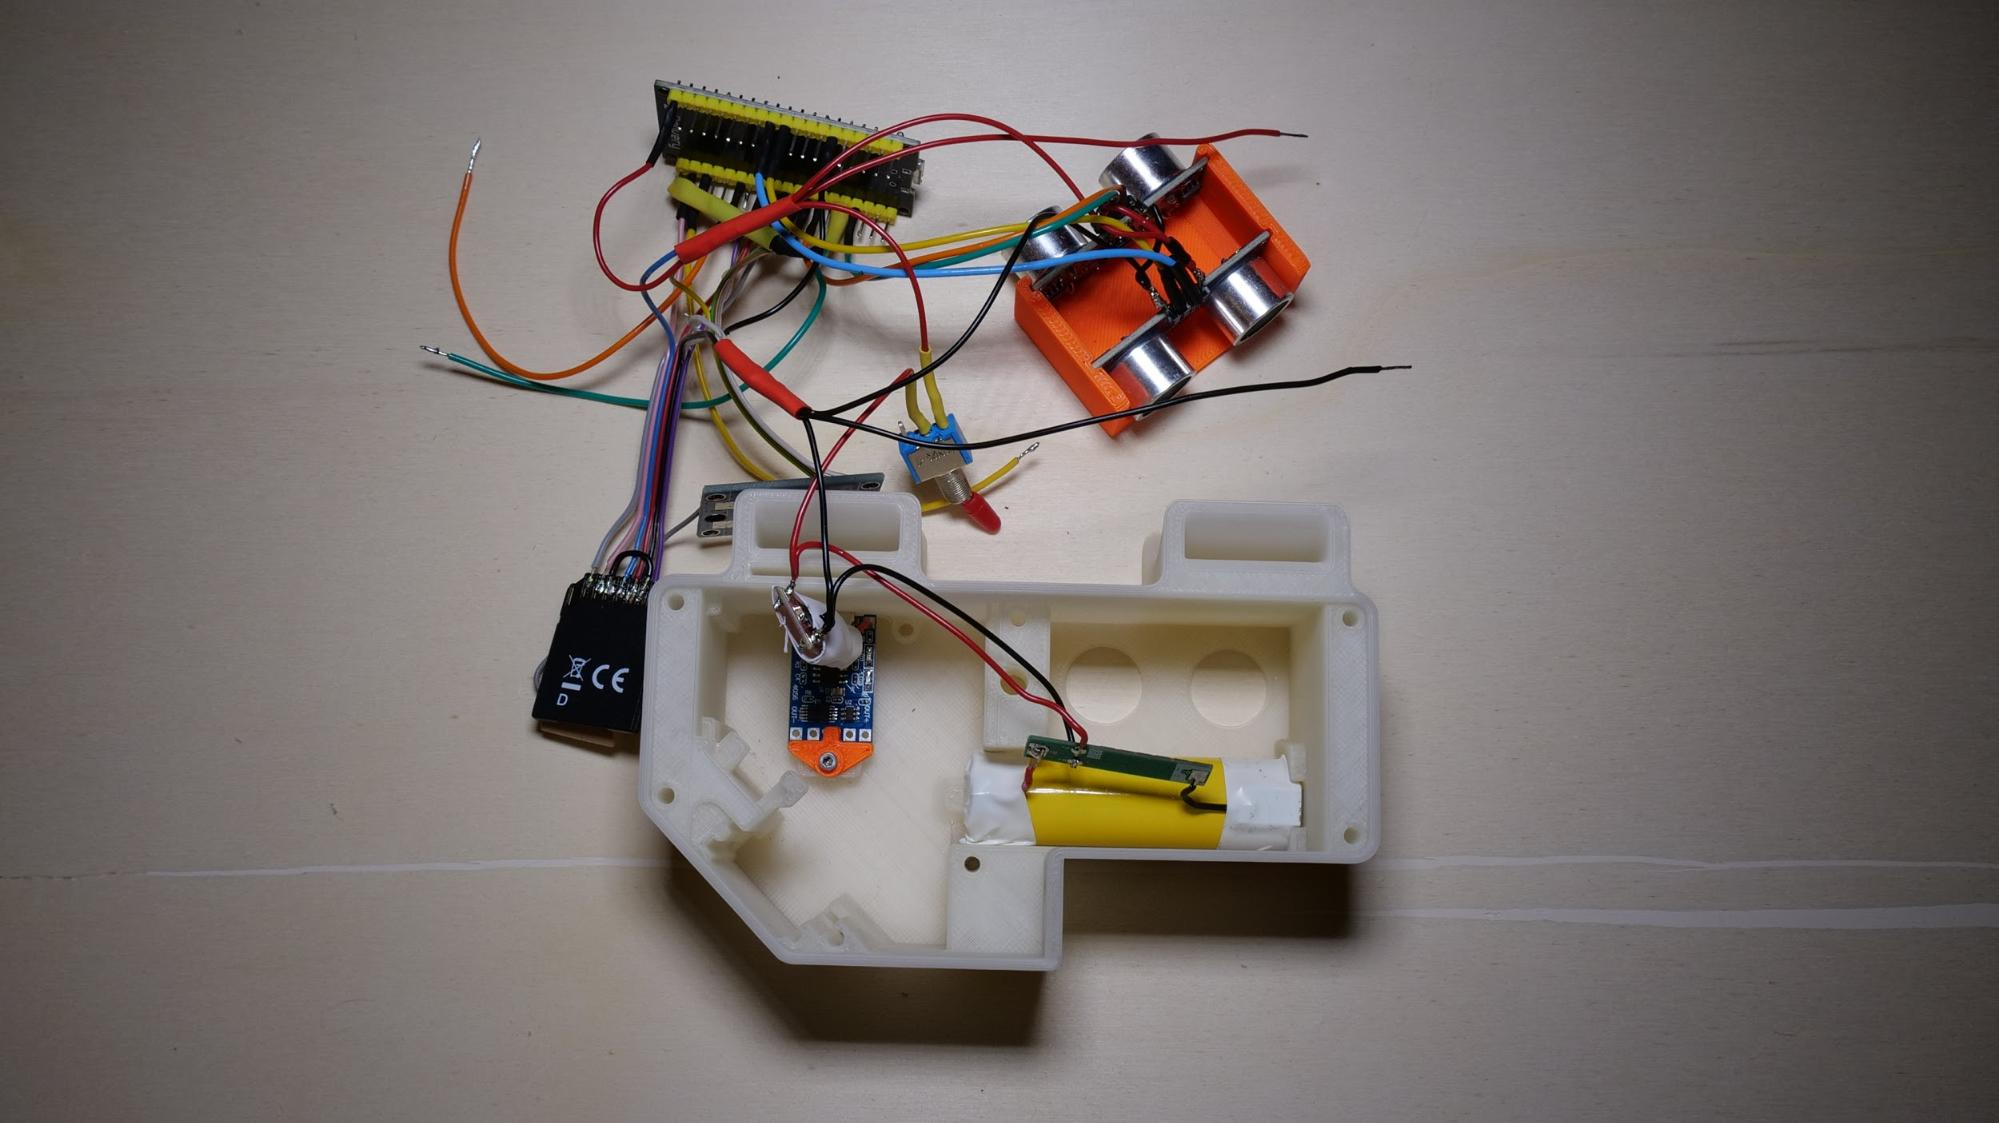
\includegraphics{images/image2.jpg}}

{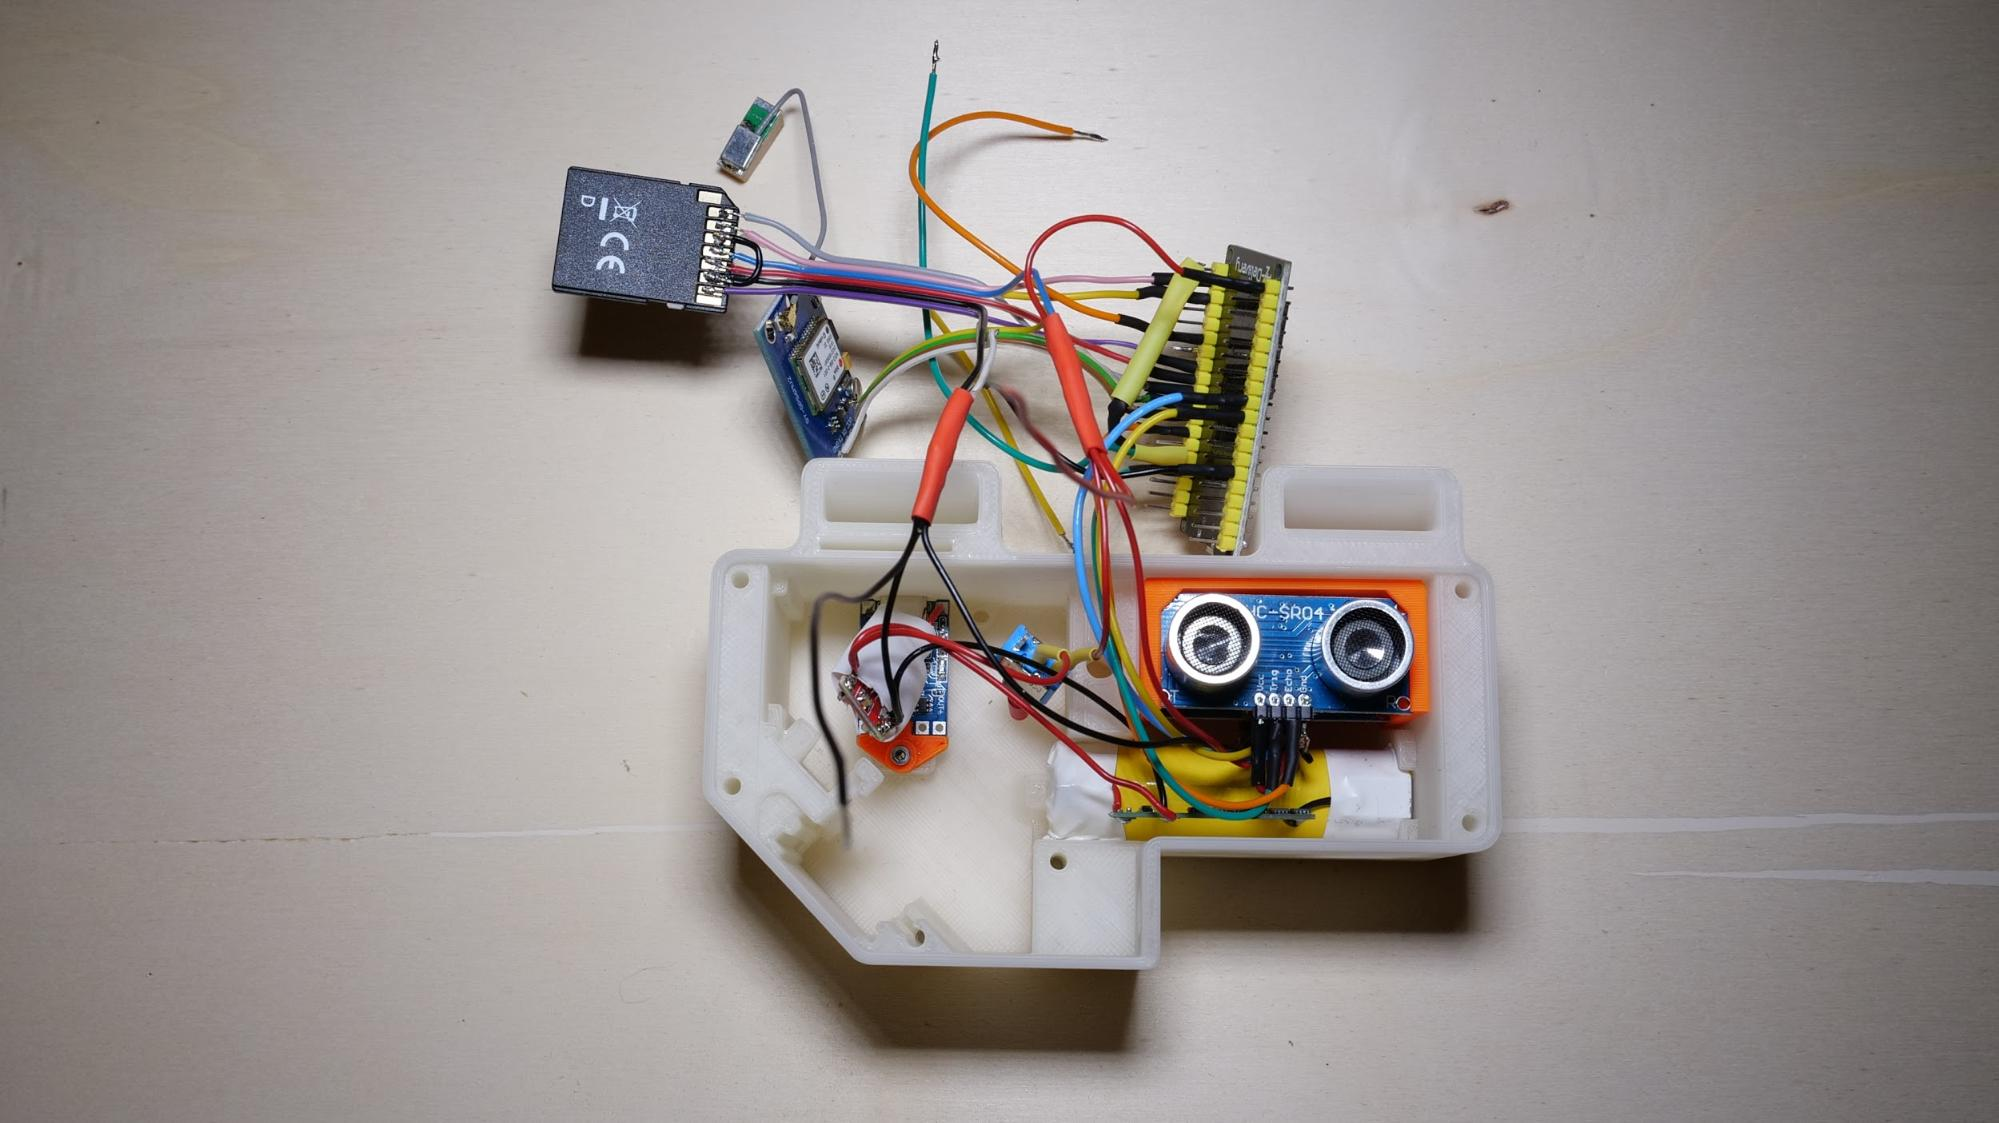
\includegraphics{images/image17.jpg}}

{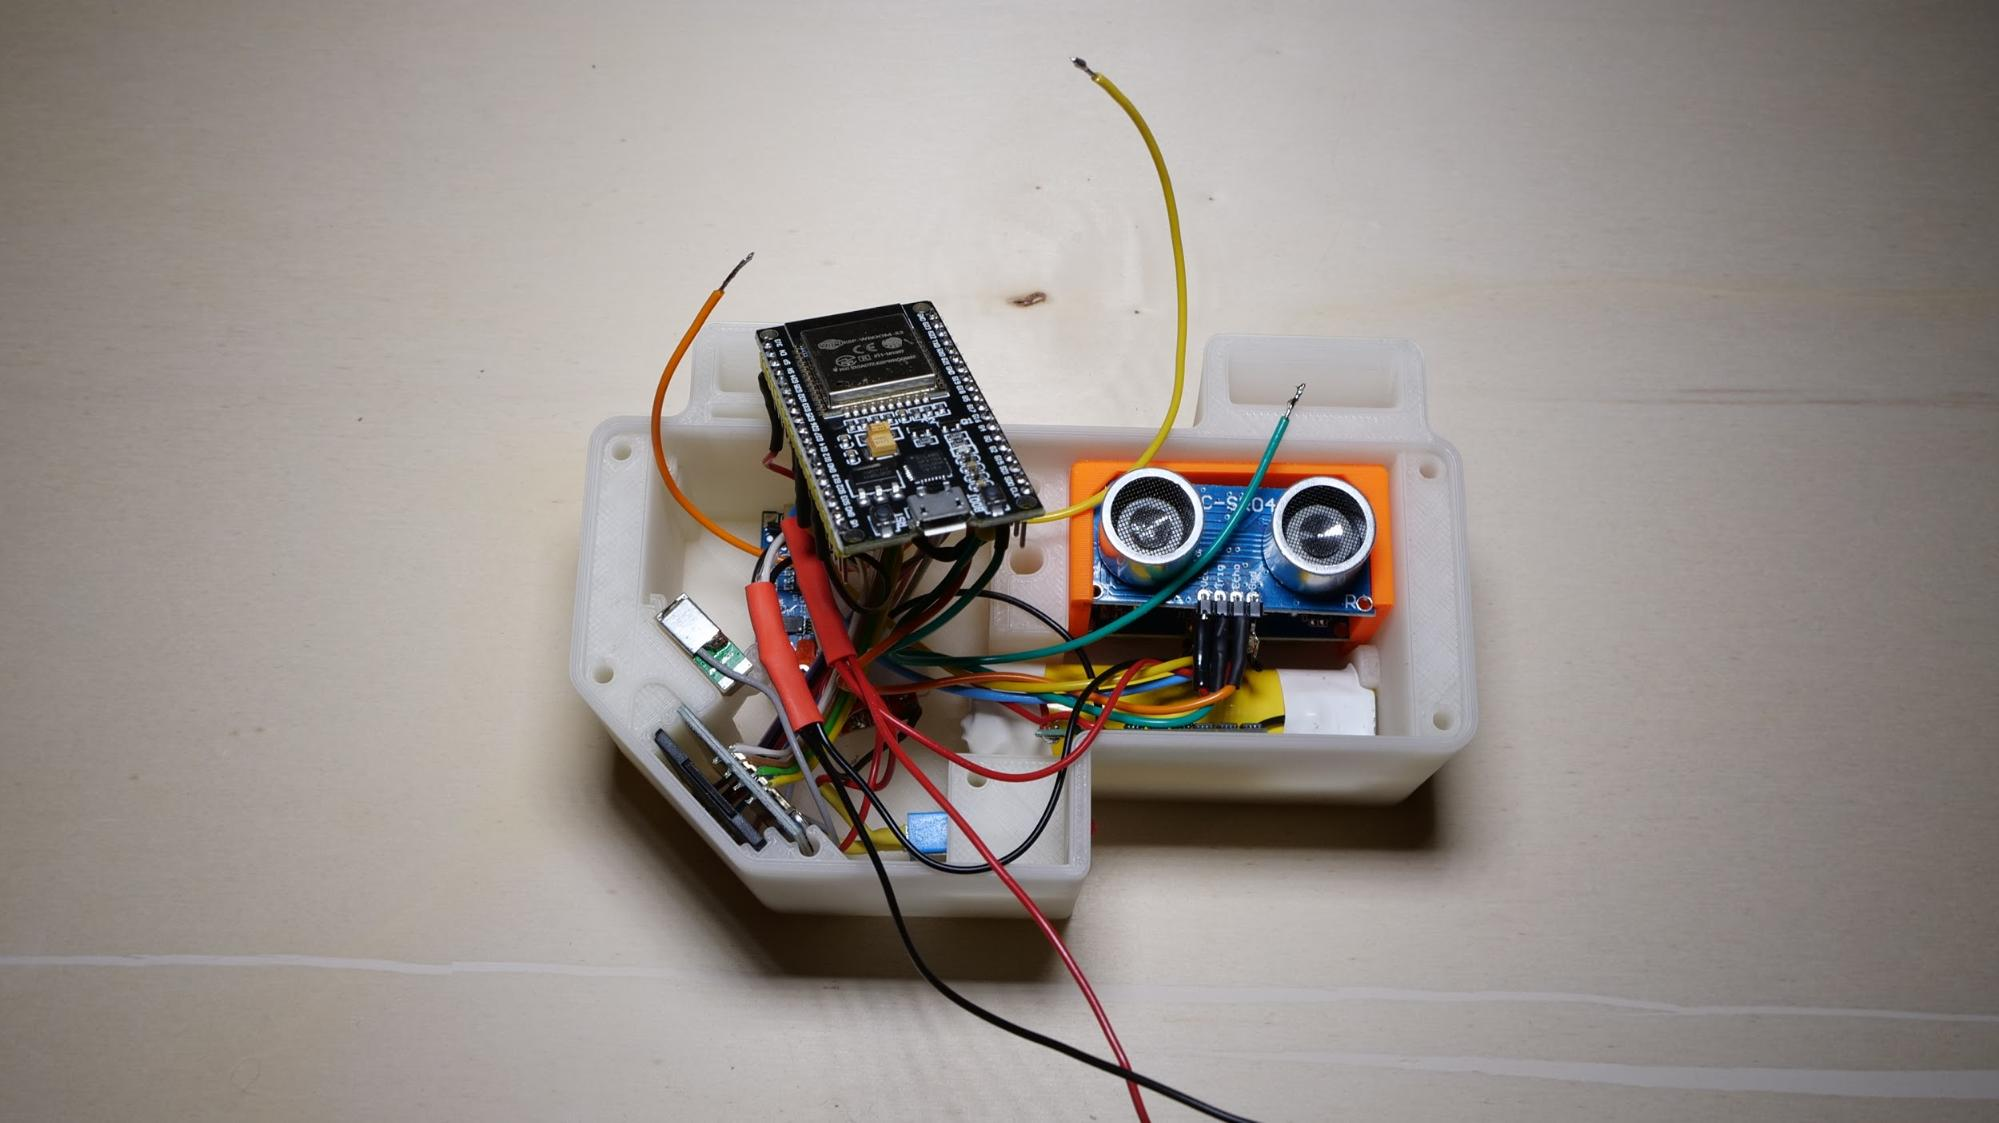
\includegraphics{images/image11.jpg}}

{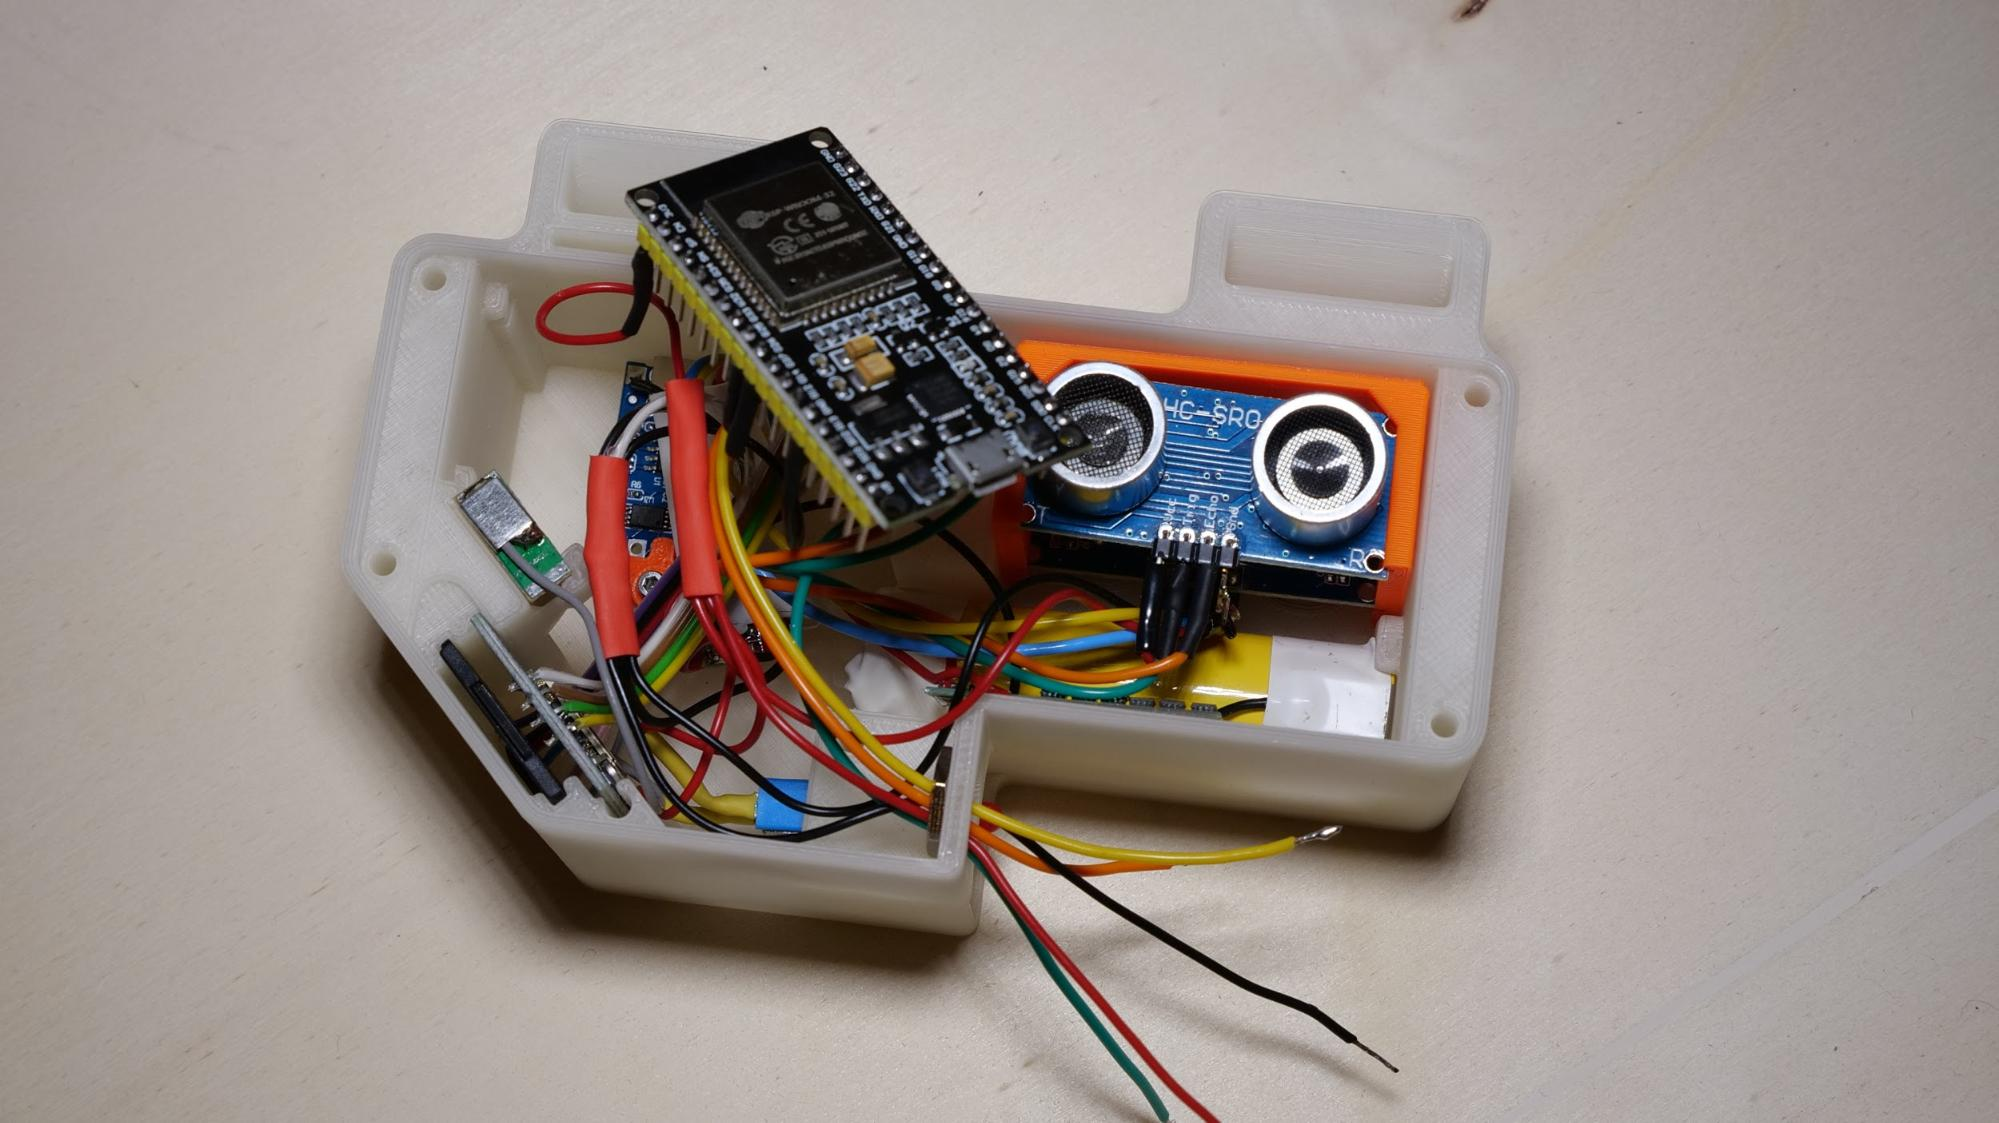
\includegraphics{images/image15.jpg}}

{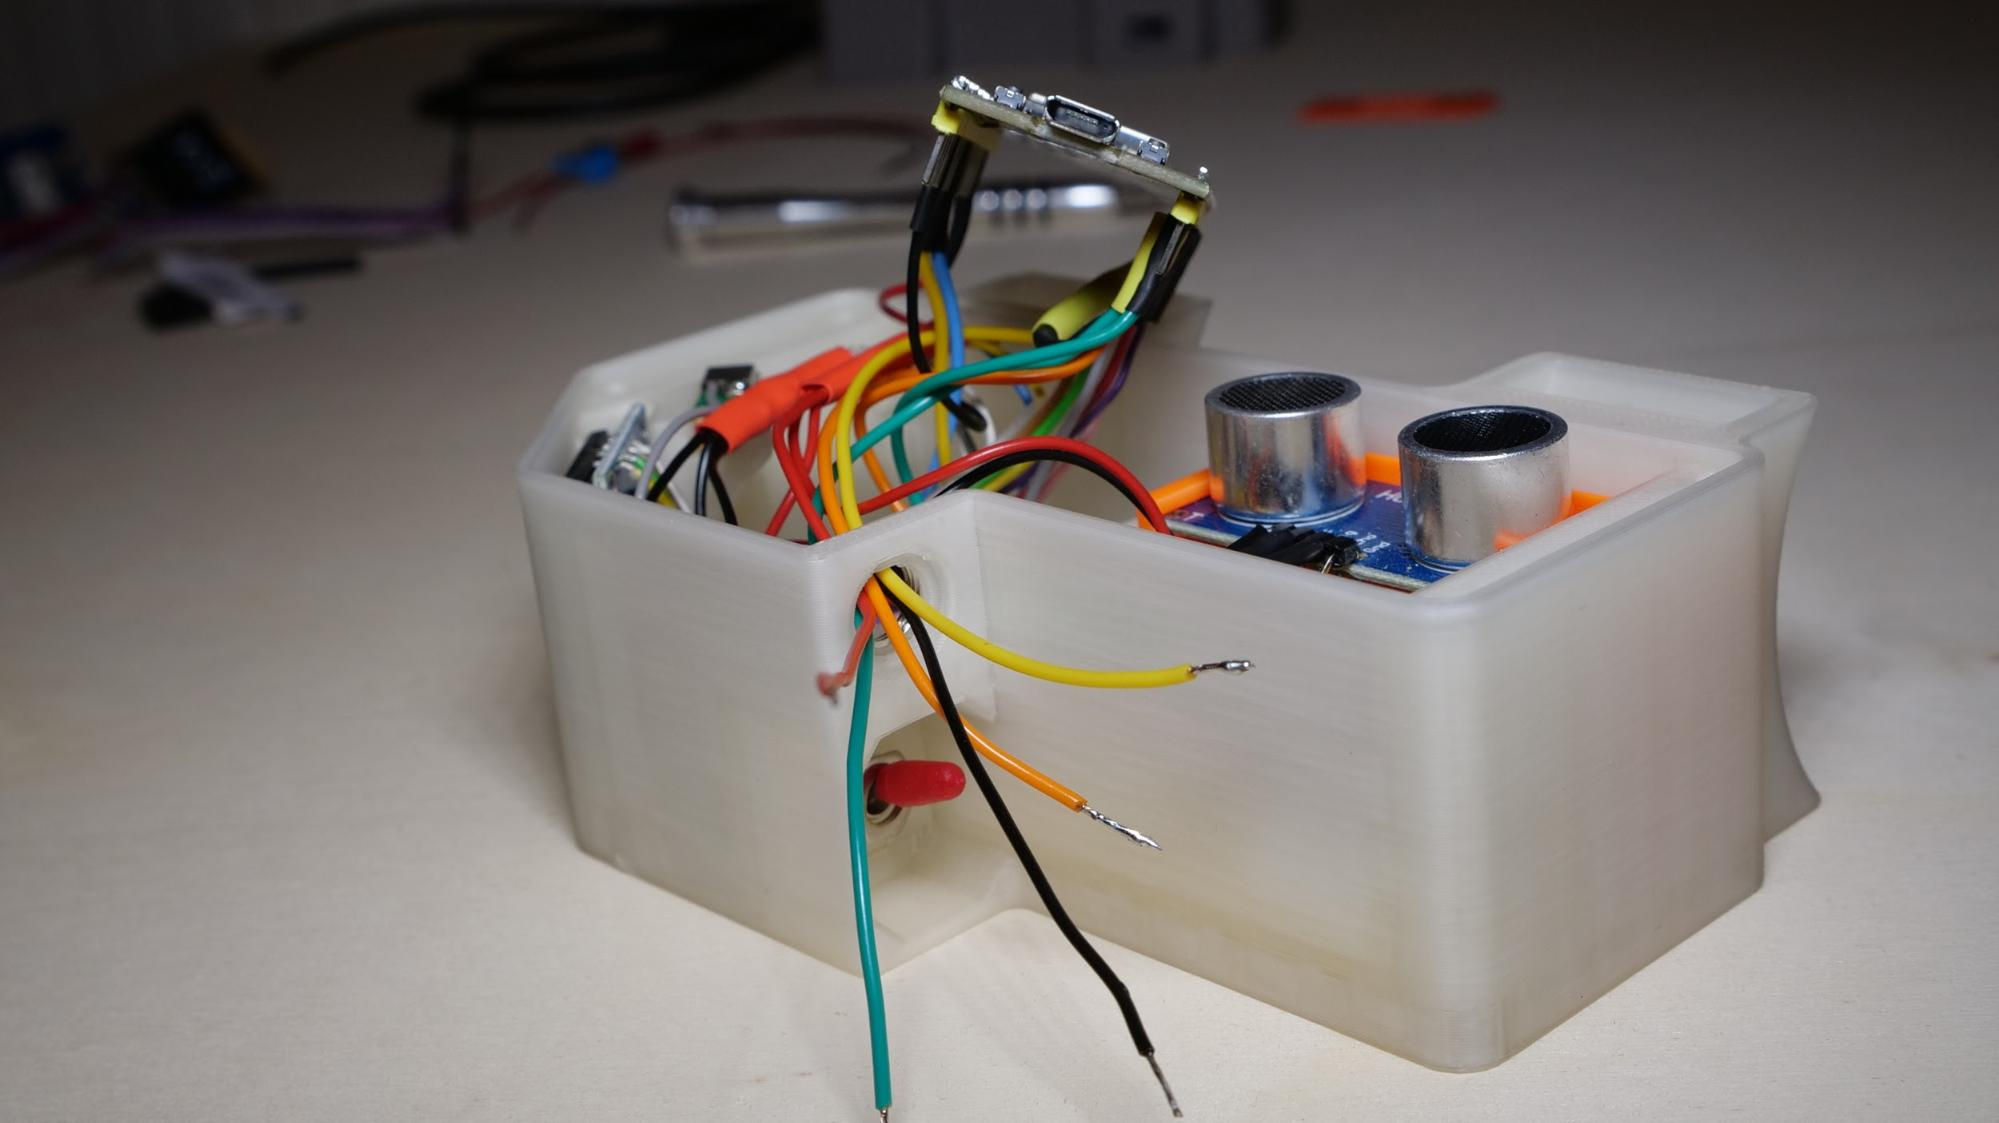
\includegraphics{images/image12.jpg}}

{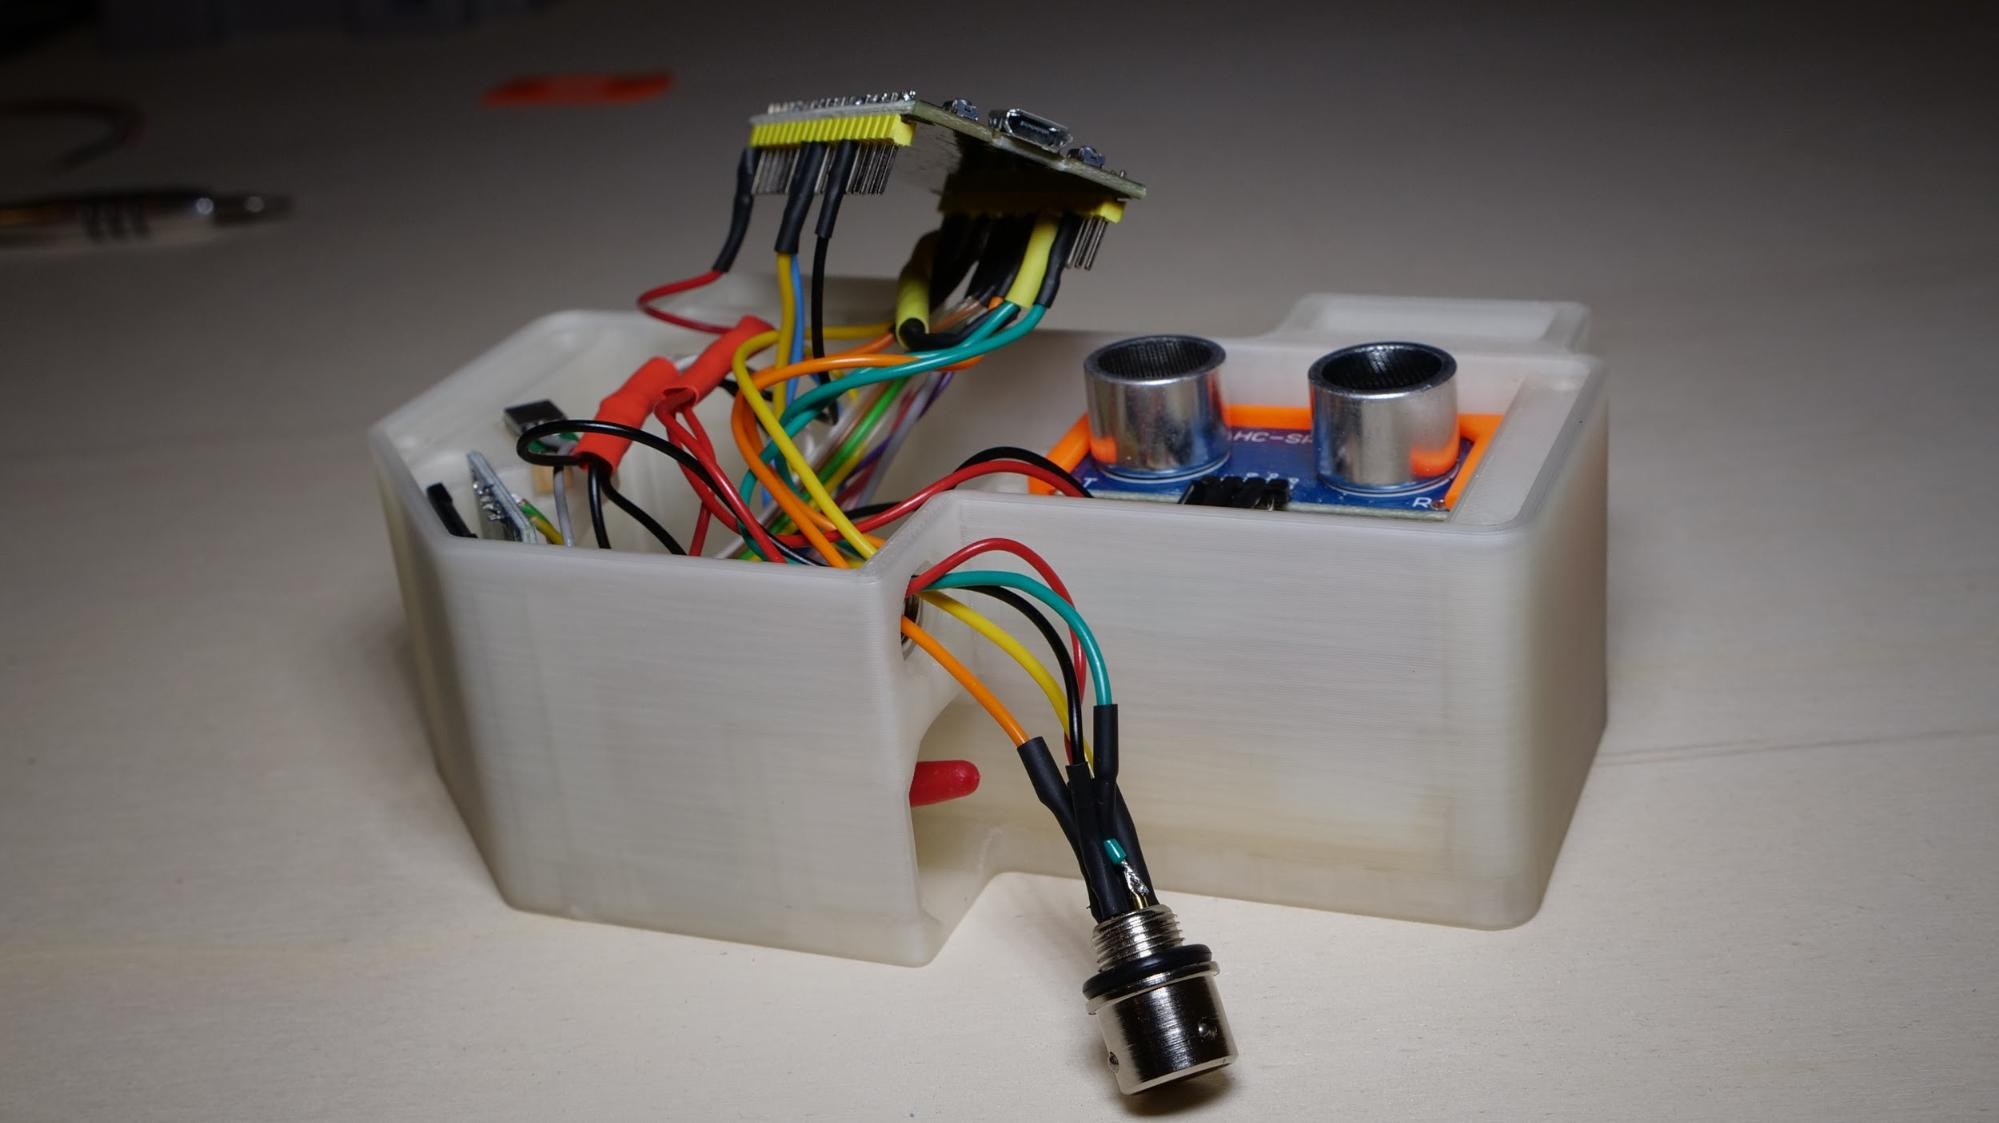
\includegraphics{images/image7.jpg}}

{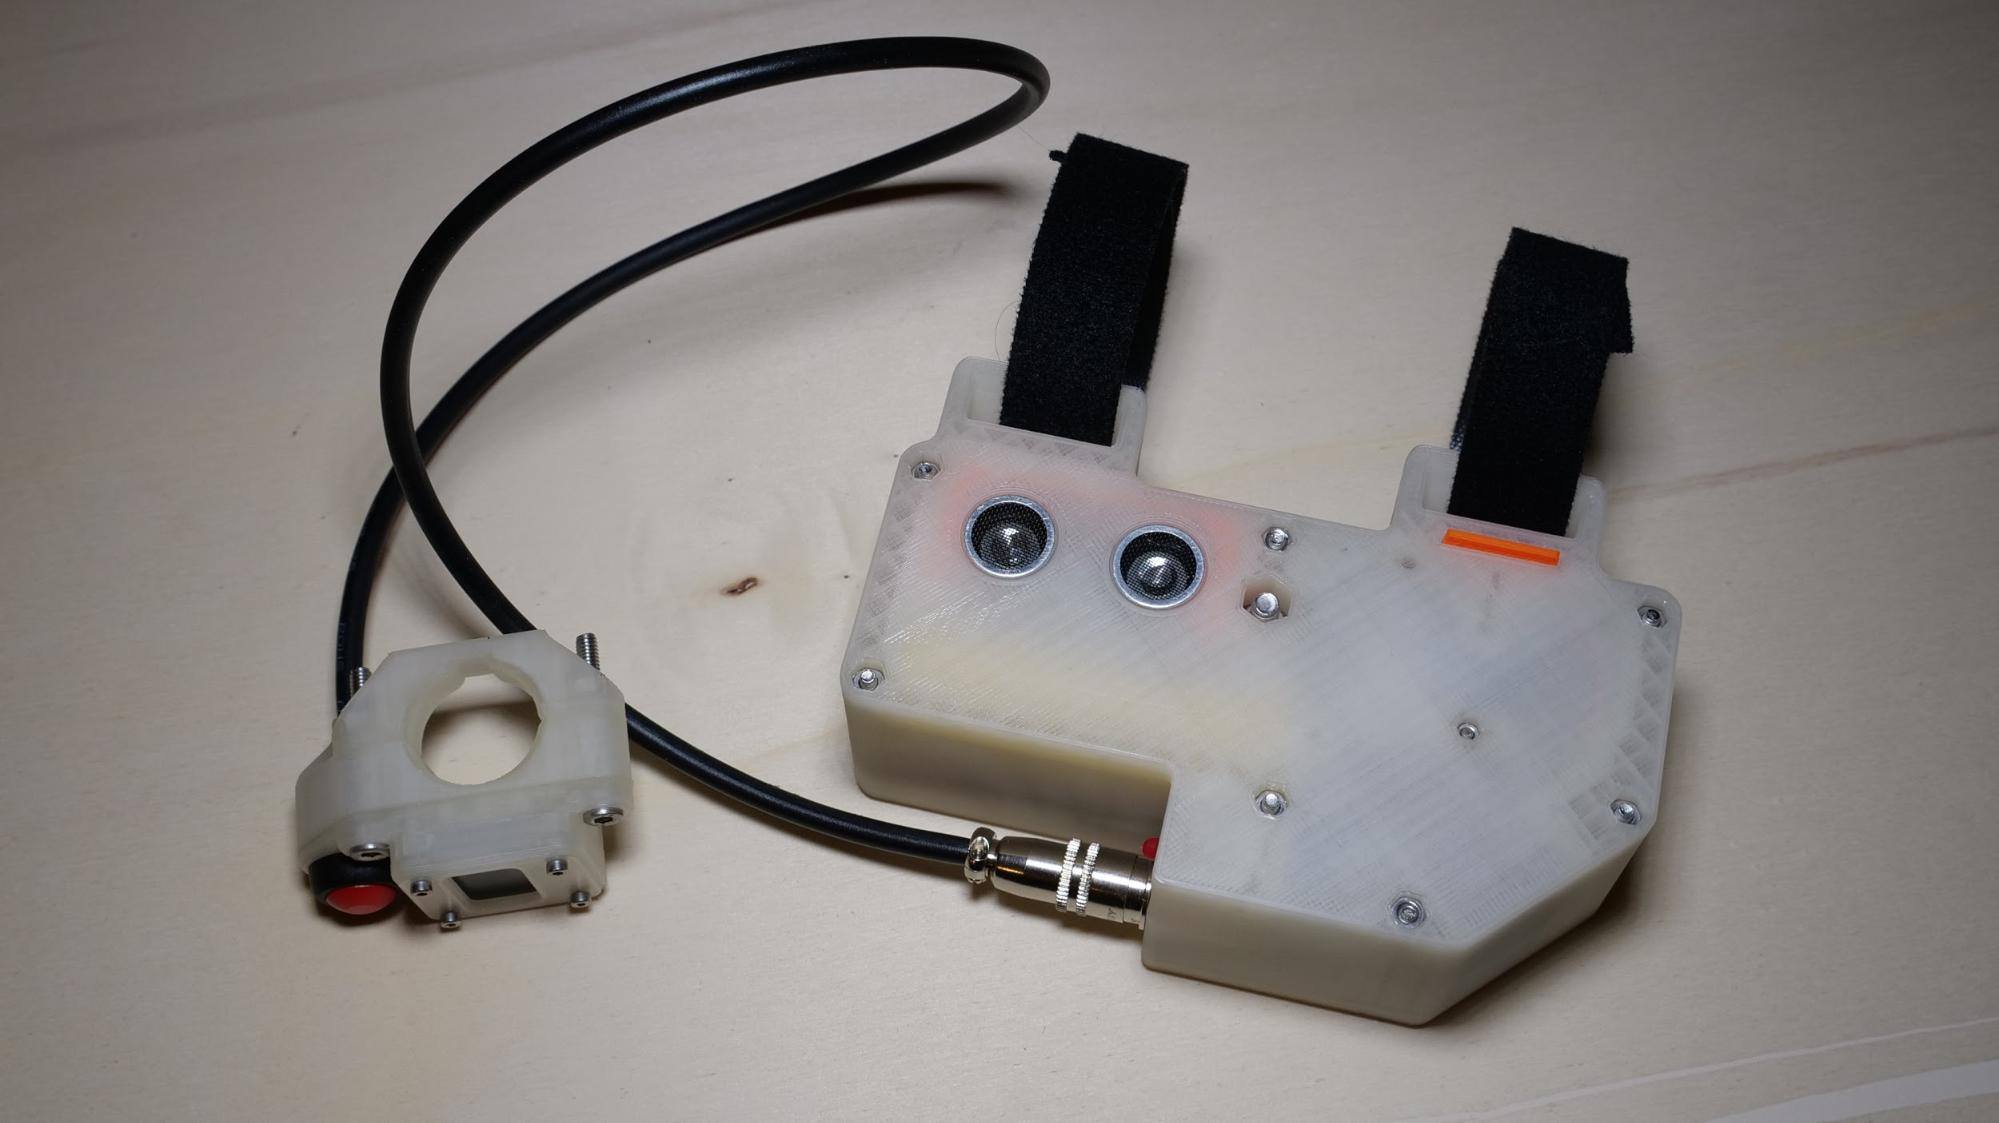
\includegraphics{images/image13.jpg}}

{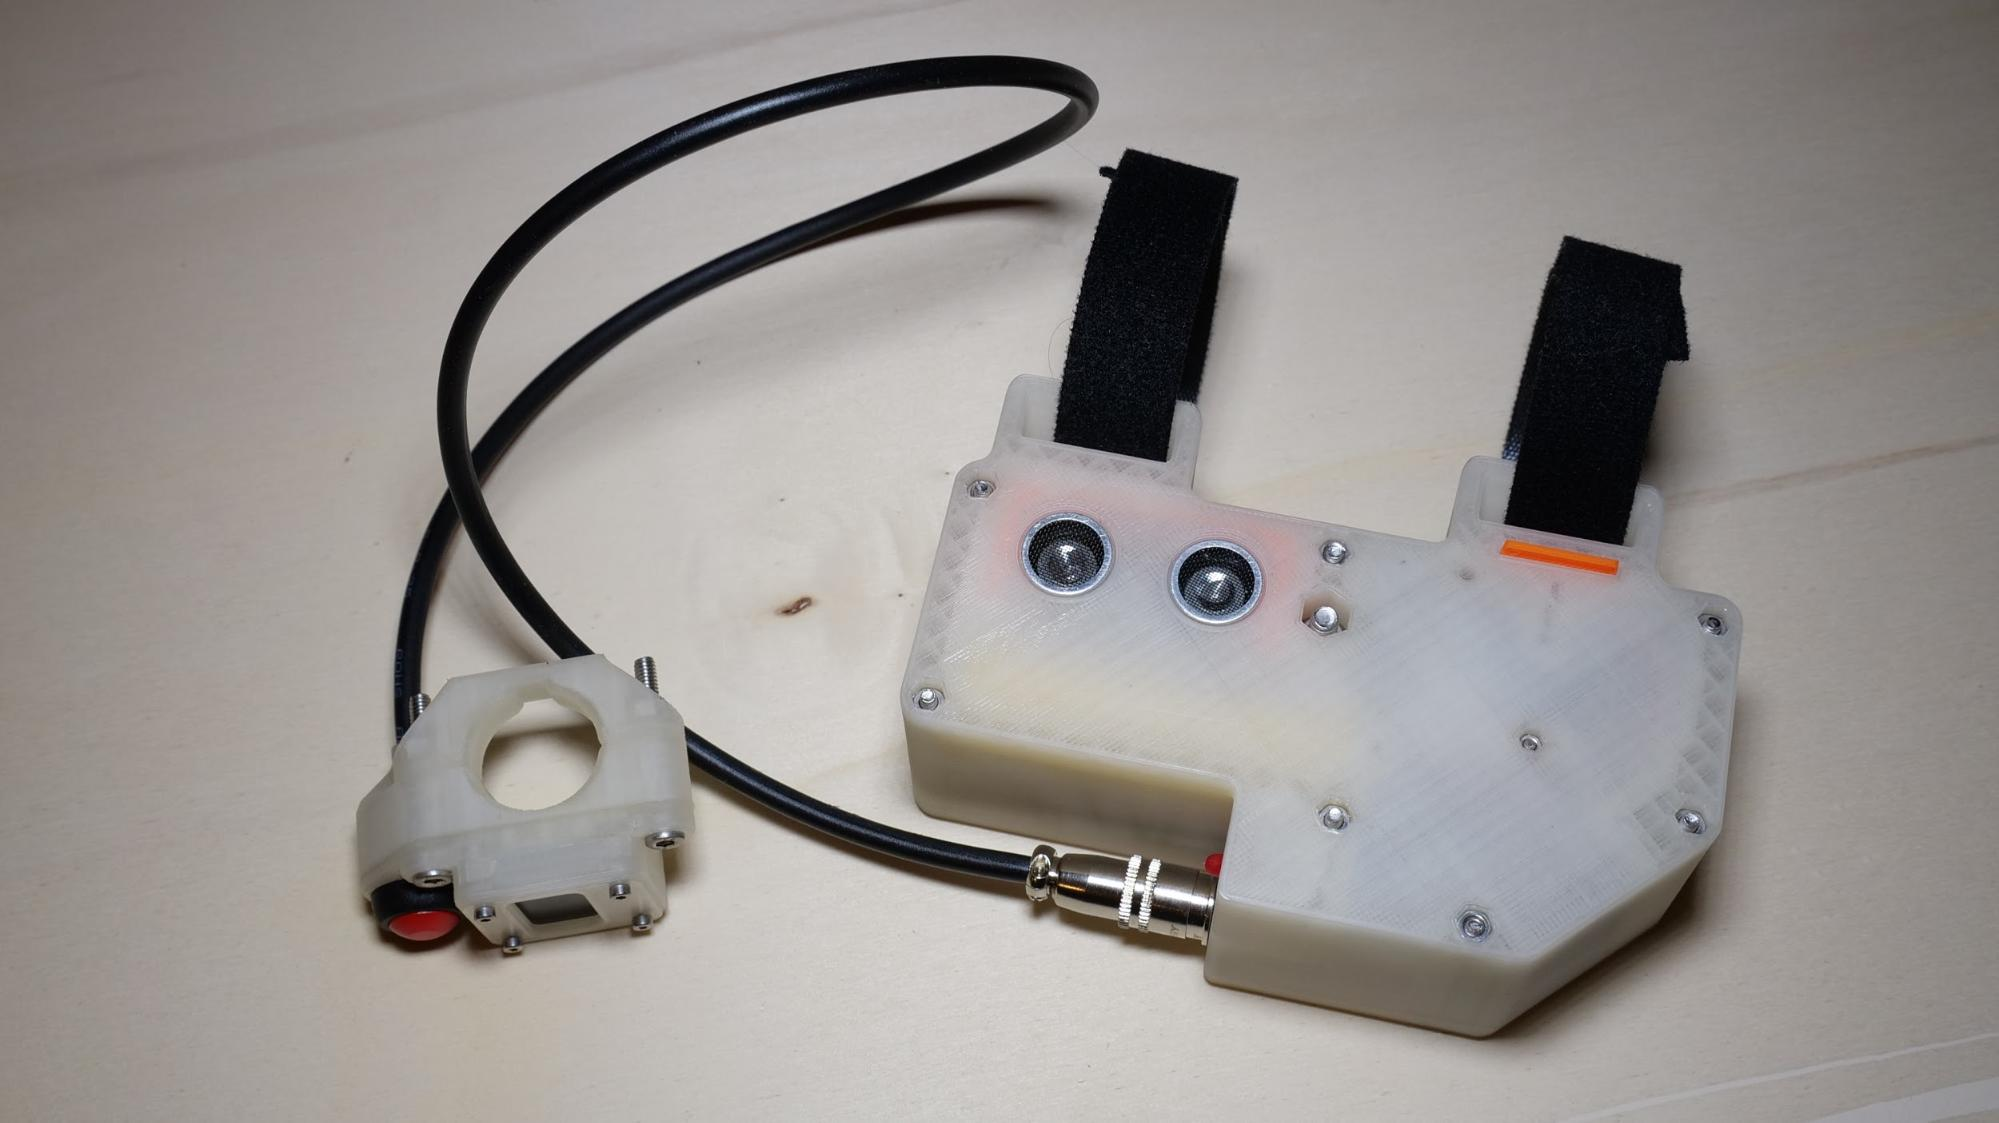
\includegraphics{images/image10.jpg}}


\end{document}
